\documentclass{article}
\usepackage[utf8]{inputenc}
\usepackage[margin=2cm,tmargin=2.5cm, footskip = 20pt, voffset=-0.3in]{geometry}
\usepackage{hyperref}
\usepackage{graphicx}
\usepackage{parskip}
\usepackage[skip=5pt, width=0.75\textwidth]{caption}
\usepackage{subcaption}
\usepackage{amssymb, mathtools}
\usepackage{algorithm}
\usepackage{algpseudocode}
\usepackage{comment}
\usepackage{appendix}
\usepackage{multirow}
\usepackage{multicol}

\setlength{\parindent}{0pt}
\title{Space Py Quest}
\author{Isobel Romero-Shaw and Roshni Vincent \\
{\small With thanks to Phillip Jones and Andreas Freise} \\
Issue 0.1}
\date{\today}

\begin{document}

\maketitle
\hrule
\tableofcontents
\hrule
\clearpage

\section{Introduction}
\label{sec:introduction}
Space Py Quest is an interferometer range-optimisation game based on
Space Time Quest. Space Py Quest aims to enhance the educational
capacities of Space Time Quest by providing users with the opportunity
to examine and alter the code themselves. The two have similar
underlying mechanics, but the methods by which a user interacts with
each encourage different learning outcomes. 

Space Time Quest is available as an application (`app') on the App
Store, Google Play, or at \url{www.laserlabs.org}. The equations used
in Space Py Quest are identical to those used in Space Time Quest, up
to some arbitrary scaling factors that prevent the games giving
identical results. Without these changes, users could numerically test
Space Py Quest's code to find Space Time Quest's high scores, making
its leaderboard redundant as a motivational goal for the
game. Space Py Quest is intended to be open-source, interfacing to a
game-player through a Jupyter notebook \cite{jupyter} with an
auto-updating plot that adjusts according to the detector parameters
set using iPython widgets \cite{ipy}. It has been written in Python
because this high-level language is widely familiar and accessible,
allowing other students to read, understand and change the
code. Python is already being taught in primary schools, making
Space Py Quest an ideal teaching tool for the future.

This document fills the gap between both Space Quest games and actual
sensitivity modelling software. Space Py Quest's noise curves have the
same scaling and overall shape of their real counterparts, but the
functions that it uses to obtain them are accessible to the user
through the code, and referenced and explained within this
text. Space Py Quest should be simple enough to adjust that it can be
successfully understood and played within a timeframe short enough to
entertain, but not bore, its player. Thus, although the functions used
to generate noise curves are \textit{based} on physically correct
equations, they are simplified to avoid over-complicating the game. An
average user, for example, will benefit from learning that less excess
gas leads to more detections, and may be interested to know that this
is to do with the gas particles interrupting the laser beam; they are
less likely to want to know exactly how the velocity of each particle
affects the  residual gas noise curve.

In this document, the simplified equations and simplifying assumptions
employed by Space Py Quest are referenced and explained. 
Section \ref{sec:theory} provides the equations used by the game to
calculate the detector range and, in the process, generate its noise
curves. Section \ref{sec:making} describes the making of the game
code. Section \ref{sec:testing} details the testing of Space Py Quest,
achieved by ensuring that the noise curves and parameters behave as
dictated by the noise equations and realistic expectations. Ideas for
future development of the game are given in the discussion in section
\ref{sec:discussion}. Any utility functions used by the code and all
constants referenced in equations presented in this document are
provided in the appendix. 


%\begin{comment}
If this is the internal copy of the Space Py Quest documentation, then
section \ref{sec:changes} will summarise exact changes made to
arbitrary factors in order to distinguish Space Py Quest's results
from those of Space Time Quest. If not, both this section and this
sentence should be commented out. 
%\end{comment}

\subsection{Differences between Space Time Quest and Space Py Quest}
\label{sec::differences}
Space Time Quest is designed to be played by a wide range of mostly
non-experts, who are motivated to get the best score by beating their
friends or winning a place on the leaderboard. Space Py Quest can also
be played by non-experts, but is more apt for those who wish to
interact with the driving code or understand the noise curves. Some
example differences between the two games are listed and discussed
below.

\begin{enumerate}
    \item \textbf{Format} \\
    Space Time Quest is an app with eye-catching graphics and clear
    transitions between stages of the game. Space Py Quest exists
    within a Jupyter notebook, which is not as graphically
    interesting. It requires some interaction with code, with a user
    handling a set of parameters in order to initialise the detector
    as either aLIGO or LIGO Voyager. This introduces Python's
    $dictionary$ type to the player, and demonstrates how Space Py
    Quest can provide programming education in addition to the lessons
    taught by Space Time Quest. It is not yet as visually appealing,
    but this could also be something for a user to alter
    themselves. The motivation then slightly deviates from that of
    Space Time Quest - \textit{Build Your Own Detector Sensitivity
      Modelling Software} rather than \textit{Build Your Own
      Detector}.
    \item \textbf{Narrative} \\
    In Space Time Quest, the game follows the user as they set up
    their detector in a certain site, lower the sensitivity curve as
    far as possible within the budget, and run the detector to find
    their score. As such, there is a clear beginning, middle and end
    to each attempt. Space Py Quest was designed for efficiency of
    results. The user may change the site of the detector at any
    point, and may run the detector to find its range as many times as
    they like without having to restart the game. Again, this is more
    in line with a \textit{Make Your Own Detector Sensitivity
      Modelling Software} aim - whilst detectors themselves might not
    be easy to change once built, detector designs are flexible and
    cost-effective ways of trialing new ideas.
    \item \textbf{Removable Noise Curves} \\
    Users of Space Py Quest are able to choose which noise curves are
    displayed using tick-box widgets, allowing the effects of
    different parameters on individual noise sources to be
    investigated.
    \item \textbf{Integration Methods} \\
    Space Time Quest was originally written in Java and then
    C\#. These are much faster languages, computationally, than
    Python. The Space Time Quest methods use manually-coded trapezium
    integration, which make Space Py Quest painfully slow to run and
    update. Using this kind of integration would have made the Markov
    chain Monte Carlo analysis, discussed in section \ref{sec:mcmc},
    extremely inefficient. Instead, Space Py Quest makes use of the
    SciPy library's Simpson's integration function,
    $scipy.integrate.simps$. Using a different integration method has
    lead to  slight discrepancies between Space Time and Space Py Quest's outputs.
\end{enumerate}

%\clearpage
\section{Theory Behind the Game}
\label{sec:theory}
\subsection{Detector Score Calculations}
\subsubsection{Detector Range}
In Space Py Quest, the detector range is the distance to which the
detector can observe mergers of two given masses, $m_1$ and $m_2$,
based only on the inspiral section of their signal. During this stage
of the coalescence, the signal amplitude spectral density in the
frequency domain has roughly the same gradient as the total noise
amplitude spectral density, and goes as $f^{-7/3}$ \cite{ajith}. The
merge and ringdown sections of the signal, which occur at higher
frequencies, are not considered in this calculation. This has the
effect of rendering the high-frequency sensitivity of the Space Py
Quest detector irrelevant to the detector range for heavier masses,
whose inspiral signal terminates at relatively low frequencies within
the detector's frequency band.

The net noise power spectrum, $\mathcal{S}$, is the sum of the squares
of all noises at each point in the detector's sensitive frequency
band.
    The \textit{sensitivity integral} is the integral of the signal-to-noise ratio,
    \[
    \mathbf{I}_S(f) = \int_{f_{lo}}^{f_{hi}} \frac{f^{-\frac{7}{3}}df}{\mathcal{S}},
    \]
    where $f_{lo}$ and $f_{hi}$ denote the lower and upper limits of the frequency range, respectively.
    The Keplerian frequency at the innermost circular orbit of a binary inspiral is
    \begin{equation}
    \label{eq:isco}
    f_{isco} = \frac{1}{6^{1.5}\pi(m_1+m_2)M_{\odot,nu}},
    \end{equation}
    Where $M_{\odot,nu} = \frac{M_{\odot}G}{c^3}$ is the Sun's mass in
    natural units. At $f_{isco}$, which point the gravitational wave
    inspiral signal stops for lower masses, and transitions into the
    actual merge and then ringdown signals for more massive
    binaries. This becomes the upper limit of the sensitivity line
    integral, $\mathbf{I}_S(f)$.

    The combined mass of the binary is defined by its chirp mass,
    \[
    \mu = \frac{(m_1m_2)^{0.6}}{(m_1 + m_2)^{0.2}}M_{\odot,nu}.
    \]
    The detector distance is then calculated by
    \[
    \mathcal{D} = \frac{\sqrt{\mathbf{I}_S(f) \times \mathcal{M}}}{2.26 \times Mpc_{nu}},
    \]
    where
    \[
    \mathcal{M} = \frac{80\mu^{\frac{5}{3}}}{96\pi^{\frac{4}{3}}\tau_{snr}^2}.
    \]
   and $\tau_{snr} = 8$ is the signal-to-noise ratio required for
   observation. $Mpc_{nu} = \frac{Mpc}{c}$ is Mpc in natural
   units. The equation for $\mathcal{D}$ is used to find the ranges to
   which the detector can observe binary black hole mergers,
   $r_{bhbh}$, and binary neutron star mergers, $r_{nsns}$. For the
   black holes, both masses are taken as 47 $M_{\odot}$, whilst for
   neutron stars, the masses are both 1.7 $M_{\odot}$.

\subsubsection{Detector Cost}
The total cost, $\mathcal{C}$, is the sum of parameter-dependent
costs, $C_i$. Its dependence on the number of suspension stages $N_s$,
suspension length $l$, and mirror mass $M$ is contained within the
component that considers vibration, $C_{vib}$. There is also a
dependence on mirror mass in the calculation of the roughness cost,
$C_r$, which is influenced additionally by the mirror roughness $R$
and the roughness losses $\mathcal{L}_R$. The laser power, $P$, and
detector depth, $d$, contribute costs $C_{pow}$ and $C_{depth}$
respectively. The cooling cost, $C_{temp}$, is dependent on the
detector temperature $T$, its initial ambient temperature $T_0$, the
temperate change, $\Delta T$, per kilometer, and the temperature of
nitrogen, $T_N$. These costs are calculated as given below.
    \[C_{depth} = \begin{cases}
                  (d-20)^{\frac{1}{3}} \times 75 \times 10^5 & \text{when $(d-20) > 0$} \\
                  0 & \text{otherwise}
                  \end{cases}
    \]
    
    \[C_{temp} = \begin{cases}
                 A_{T, 1}\times\left(T_0 + \frac{d\Delta T}{100} - T\right) & \text{when $T > T_N$} \\
                 7 \times 10^6 + A_{T, 2}\left(77 - T\right)^2 & \text{otherwise}
                 \end{cases}
    \]
    \[
    \text{(where arbitrary constants $A_{T, 1}$ and $A_{T, 2}$ are 20102 and 10201, respectively)}
    \]
 \begin{multicols}{2}   
    \[C_{Np} = N_p \times C_v
    \]

        \[C_{r} =\frac{M^{\frac{2}{3}}(R^3 - \mathcal{L}_R^3)(8 \times 10^7)}{25}
    \]
    \break
    \[C_{mat} = \mathcal{C}_{mat}
    \]

    \[C_{pow} = 47 \times 10^3 + 25 \times 10 ^ 6 \times \left(\frac{P}{P_{hi}}\right)^2 
    \]
    \[
    \text{(where $P_{hi}$ is the upper power limit)}
    \]

    \[C_{vib} = l^{a_v} \times N_s^{b_v} \times M^{c_v} \times 60 - 60
    \]
    \[
    \text{(where $a_v$, $b_v$ and $c_v$ are 2.1, 5.5 and 1.2 in that}
    \]
    \[
    \text{order, and $a_v$ and $c_v$ are arbitrary)}
    \]
 \end{multicols}   

Then
\[
\mathcal{C} = \sum_{i} C_i,
\]
where $i$ represents a parameter with a unique cost.
\subsubsection{Numbers of Detections (and Missed Detections)}
\begin{itemize}
\item\textbf{Binary Neutron Star Mergers}\\
    The number of black hole binary merge signals detected is the rounded result of
    \[
    N_{nsns} = \frac{4\pi\times6000}{3 \times 12}\left(\frac{r_{nsns}}{1 \times 10^3}\right)^3 ,
    \]
    where $r_{nsns}$ is the range to which the detector can sense
    neutron star mergers with component masses of 1.7 $M_{\odot}$.
\item\textbf{Binary Black Hole Mergers}\\
    The number of neutron star binary merge signals detected is the rounded result of
    \[
    N_{bhbh} = \frac{4\pi\times20}{3 \times 12}\left(\frac{r_{bhbh}}{1 \times 10^3}\right)^3 ,
    \]
    where $r_{bhbh}$ is the range to which the detector can sense
    black hole mergers with component masses of 47 $M_{\odot}$.
\item\textbf{Supernovae}\\
    Detectors with good mid- to high-frequency sensitivity can obtain
    just \textit{one} supernova detection. This was done after the
    tests described in section \ref{sec:mcmc} were performed. The
    supernova signal amplitude curve is found using the total noise
    amplitude curve $\mathcal{S}$,
    \[
    y_s = \sqrt{\mathcal{S} + (1 \times 10^{-23})^2}.
    \]
    The area under both the noise and the supernova curves is
    calculated by taking their integrals, $\mathcal{I}_n$ and
    $\mathcal{I}_s$ respectively. The result is then
    \[
    N_{sn} = \begin{cases}
             1 & \text{if $25 \times \left(\frac{\mathcal{I}_s - \mathcal{I}_n}{4 \times 10^{-20}}\right)^3 \geq 1$} \\
             0 & \text{otherwise}.
             \end{cases}
    \]
\item\textbf{Complexity}\\
The `complexity', $\mathcal{Z}$, is a measure of how challenging it is
to maintain the detector. If a detector requires a lot of time to
restore it to its design sensitivity when it breaks, then it spends
less time observing, and events can be missed as a result. The
\textbf{total} complexity is the \textbf{sum} of complexities due to
the detector's depth $d$, and temperature $T$, the number of vacuum
pumps $N_p$ and suspension stages $N_s$, the laser power $P$, and the
mass $M$, material damping rate $\mathcal{L}$, and roughness $R$ of
the mirrors. The complexities are:
        \[Z_{temp} = \begin{cases}
                     1 - \frac{T - T_N}{T_0 + \frac{d\Delta T}{100} - T_N} & \text{ when $T > T_N$} \\
                      5 & \text{otherwise}
                     \end{cases}
        \]
\begin{multicols}{2}   
        \[Z_{r} = 1 + \frac{50 - R}{500}
        \]
        
        \[Z_{Np} = \frac{N_p}{10}
        \]

        \[Z_{Ns} = \frac{N_s}{2}
        \]
        \break
        \[Z_{pow} = \frac{P}{10}
        \]

        \[Z_{mass} = \frac{M}{50}
        \]
        
        \[Z_{mat} = \mathcal{L}
        \]
\end{multicols}  
Then
\[
\mathcal{Z} = Z_{depth} + \sum_{i} Z_i,
\]
where the complexity due to the detector's depth, $Z_{depth}$, is a
linear interpolation of approximated depth and complexity data, and
$i$ represents a source of complexity.
\item\textbf{Missed Detections}\\
    The number of missed events depends on the complexity of the
    detector, $Z$, itself in relation to the complexity credits of its
    site, $Z_{cred}$. The \textit{overcomplexity}, $\mathcal{O}$, is
    \[
    \mathcal{O} = \begin{cases}
                  Z - Z_{cred} & \text{if $ Z - Z_{cred} > 0$} \\
                  0 & \text{otherwise}
                  \end{cases}.
    \]
    The complexity \textit{scale}, $S_{Z}$, is then
    \[
    S_{Z} = 1 - \frac{\mathcal{O}}{Z_{cred}}.
    \]
    The number of missed sources of a given type $i$ is the rounded-down result of
    \[
    N_{missed, i} = \begin{cases}
                    N_i \times (1 - S_Z) & \text{if $N_i \times (1 - S_Z) > 0$} \\
                    0 & \text{otherwise}.
                    \end{cases}
    \]
\end{itemize}
\subsection{Noise Curves}
\begin{figure}
\centering
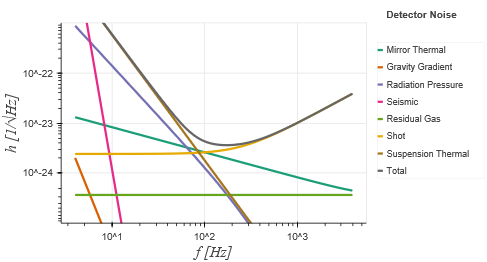
\includegraphics[width=0.8\textwidth]{SPQ_aLIGO.png}
\caption{The default aLIGO noise curve model generated by Space Py
  Quest. This detector is initialised at a depth, $d$, of 0 m, in the
  desert site, with silica mirrors. The mirrors have a roughness, $R$,
  of 1 nm, and a mass, $M$, of 40 kg. There are 4 suspension stages,
  $N_s$, and the suspension has a length, $l$, of 35 cm. 7.5 vacuum
  pumps, $N_p$, are used and the detector temperature, $T$, is 290
  K. The laser power, $P$, is set to 125 W. Unless specified
  otherwise, illustrative noise plots for the remainder of this
  section will be for a detector with these configurations.}
\label{fig:aLIGO}
\end{figure}
Examples of the noise curves displayed by Space Py Quest are scattered
throughout this document. Figure \ref{fig:aLIGO} is an example of the
plots generated by the game, with the detector variables set as
described. Gravitational waves induce extension or compression of the
arms of the detector, which can be expressed as a fractional length
change, or strain. Strain $noise$ arises when things that are not
gravitational waves cause the detector to behave as though its arms
have been strained. In Space Py Quest, strain noise is illustrated as
an amplitude spectral density in the frequency domain, allowing the
user to view a time-averaged snapshot of the strain that the noise
sources emulate.

\subsubsection{Total Sensitivity Curve}
As displayed in figure \ref{fig:aLIGO}, the $total$ sensitivity curve
is the vector sum of the individual noise contributions. This is the
limit of the detector's sensitivity.

\subsubsection{Individual Noise Sources}
Each of these equations calculates the noise at a single frequency, $f$.
\begin{itemize}
	\item \textbf{Ground Motion Noise} \\
    \begin{itemize}
    \item \textbf{Seismic} \\
       \begin{figure}[h!]
    \centering
    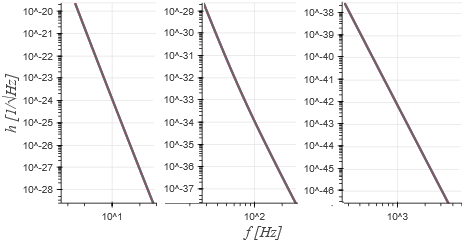
\includegraphics[width=0.6\textwidth]{SPQ_aLIGO_seismic.png}
    \caption{Approximate seismic noise model for the aLIGO detector
      described in figure \ref{fig:aLIGO}. Seismic oscillations affect
      the detector over the entire frequency spectrum, but at
      mid-frequencies and above its contribution is extremely small in
      comparison to strain noise from other sources.}
    \label{fig:seismic}
    \end{figure}
   The base seismic noise is
    \begin{equation}
    \label{eqn::baseseismic}
    X_0 = \frac{X_{dc}}{1 + \left(\frac{f}{f_c}\right)^{n_0}} + X_{hf},
    \end{equation}
    where $X_{dc}$, $X_{hf}$, $n_0$ and $f_c$ are location-specific
    parameters that are detailed in appendix \ref{sec:sites}. $X_0$
    experiences a reduction if the detector is located a distance $d$
    underground, so that
    \[
    \mathcal{R} = \frac{1}{\sqrt{1 + \left(\frac{d}{50}\right)^4}} + 0.8\times10^{-3} .
    \]
    These two terms combine to give the final displacement due to seismic activity,
    \begin{equation}
        X_{seis} = X_0 \times \mathcal{R}.
    \label{eq:Xseis}
    \end{equation}
    The seismic noise is calculated considering a highly-damped
    pendulum with $1 < Q_{pend} < 10$, where $Q_{pend}$ is the
    pendulum quality factor. Here, we assume a quality factor of
    $Q_{pend} = 5$. 
    
    The pendulum noise spectral amplitude transfer function,
    $\mathcal{T}_{pend}$, is an approximation of equation (4) in
    \cite{VIRGO},
    \[
    h_{S} = \frac{2}{L}\left(\mathcal{T}_{H}^2 + \theta_0\mathcal{T}_V^2\right)^{\frac{1}{2}}X_{seis},
    \]
    where $L$ is the detector's arm length, $\mathcal{T}_H$ and
    $\mathcal{T}_V$ represent the horizontal and vertical spectral
    amplitude transfer functions, and $\theta_0$ is the
    vertical-to-beam-axis coupling angle. $X_{seis}$ is calculated as
    in equation \ref{eq:Xseis}.
    The pendulum oscillation frequency, $f_{p}$ is given as
    \[
    f_{p} = \frac{1}{2\pi}\sqrt{\frac{g}{l}} ,
    \] 
    where $g$ is the gravitational acceleration and $l$ is the
    suspension length. We consider only $f > f_p$, since for the
    shortest pendulum we get an $f_p$ of $\sim$ 1 Hz. The transfer
    function is calculated as
    \[
    \mathcal{T}_{pend} = \frac{1}{1 + \left(\frac{f}{f_{p}}\right)^4 - \left(2 - \frac{1}{Q_{pend}}\right)\left(\frac{f}{f_{p}}\right)^2}.
    \]
        The seismic noise is then
    \begin{equation}
        \label{eqn::seismic}
        h_{S} = \frac{2}{L}X_{seis}\left(\sqrt{\mathcal{T}_{pend}}\right)^{N_s}.
    \end{equation}
    \item \textbf{Gravity Gradient (Newtonian)} \\
    \begin{figure}[h!]
    \centering
    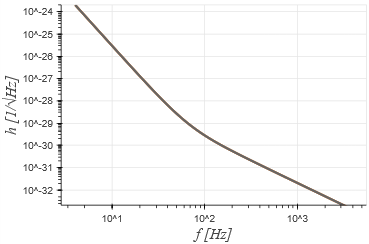
\includegraphics[width=0.5\textwidth]{SPQ_aLIGO_gravitygradient.png}
    \caption{The simplified gravity gradient noise, which becomes
      negligible to the total noise at mid to high-frequencies, but is
      a limiting contribution at low frequencies.}
    \label{fig:gravity}
    \end{figure}
    The Newtonian, or gravity gradient, strain noise arises from
    modulation to the local gravitational field due to density
    perturbations of the Earth \cite{advLIGO}. This calculation
    assumes the form of the expressions for gravity gradient noise
    given in equations (5) and (6) of the 2004 VIRGO Sensitivity Curve
    document \cite{VIRGO}. The Newtonian noise in the 2016 version of
    Space Time Quest is based on equation (6),
    \begin{equation}
    \label{eqn::GG}
    h_{GG} = \frac{X_{seis}(1.3\times10^{-8})}{Lf^2},
    \end{equation}
    where
    \[
    (1.3\times10^{-8}) \approx \frac{2.7G\rho_E\sqrt{2}}{(2\pi)^2}.
    \]
   $G$ is Newton's constant and $\rho_E$ is the density of the Earth,
   $\sim 2 \times 10^3$ kgm$^{-3}$. Equation (5) from the VIRGO
   sensitivity document returns a strain amplitude about 7 times
   larger than equation \ref{eqn::GG} here, the calculation used in
   Space Py Quest.
   \end{itemize}
   \item \textbf{Thermal Noise} \\
    \begin{figure}[h!]
    \centering
    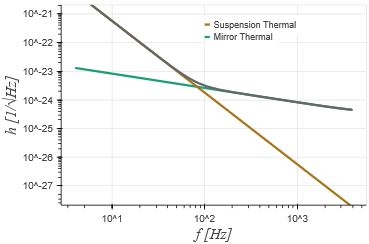
\includegraphics[width=0.5\textwidth]{SPQ_aLIGO_thermal.png}
    \caption{The thermal noise models used by Space Py Quest, which contribute significantly at the lower end of the frequency range.}
    \label{fig:thermal}
    \end{figure}
    \begin{itemize}
    \item \textbf{Mirror Thermal} \\
    The mirror thermal noise depends on the angular frequency of oscillation,
    \[
    \omega = 2\pi f.
    \]
     The correct power spectral density of the mirror's internal vibrations, as provided in \cite{VIRGO}, is
    \[
    <X_{int}>^2 = \frac{4k_bT}{\omega^2} \times\text{\textbf{Re}}\left(\frac{1}{Imp(\omega)}\right),
    \]
    where $k_b$ is the Boltzmann constant and $Imp(\omega)$ is the
    system's mechanical impedence. In order to calculate this for
    Space Py Quest, we  approximate only equation (28) from
    \cite{VIRGO}, which is used to calculate the fluctuations due to
    the first mode resonance. The expression
    \[
    w_1 = 2\pi \times A_{MT} \times \left(\frac{23}{M}\right)^{\frac{2}{3}}, 
    \]
    has been chosen to represent the first resonant frequency of the
    mirror, so that it scales inversely with mirror mass. This is
    because the Space Py Quest mirrors are assumed to maintain their
    density and aspect ratios, so higher mass means larger reflective
    surface area. $A_{MT}$ is a scaling factor, here set to 20505, and
    $M$ is the mirror mass. This gives $\omega_1$ about 4 times larger
    than those given in \cite{VIRGO} for masses of $\sim 20$ kg, but
    only about twice as large for masses of $\sim 50$ kg. 

    We use the `effective' mirror mass associated with the $w_1$ mode, $M_{eff}$,
    \[
    M_{eff} = 0.28\times M.
    \]
    This reduction follows the effective masses of $\sim 6.5$ given in
    \cite{VIRGO} for masses of $\sim 20$ kg.
    
    The Space Py Quest model returns a strain noise amplitude of
    \begin{equation}
    \label{eqn::mirror}
     h_{MT} =  \frac{4}{L}\sqrt{\frac{k_bT}{M_{eff}\mathcal{Q}}}\times\frac{w_1}{\sqrt{w\left((w_1^2 - w^2)^2 + \left(\frac{w_1^2}{\mathcal{Q}}\right)^2\right)}}.
    \end{equation}
    This incorporates our approximation of equation (28) from
    \cite{VIRGO} for the first-mode fluctuations into the relevant
    strain calculation given in equation (29).
    
    \item \textbf{Suspension Thermal} \\
    In reality, the suspension wires contribute $pendulum$
    (horizontal) oscilliations, $vertical$ oscillations, and violin
    modes \cite{violin} to the thermal noise. As in equations (19),
    (22) and (24) in \cite{VIRGO}, each contribution has the form
    \begin{equation}
    \label{eq:st}
    h_{ST} = \frac{2}{L}\sqrt{X_{ST}^2}, 
    \end{equation}
    where $X_{ST}$ are the thermal fluctuations in the suspension
    material and $L$ is the detector's arm length. We initially make
    the simplifying assumption that all suspension stages are the
    same, and that the last stage is the only one contributing to the
    thermal noise. We also assume that there are 4 suspension stages
    and that the wires are made of steel, as in the VIRGO design
    document \cite{VIRGO}. Finally, the violin modes are not included
    for simplification. 
    Thus, the Space Py Quest calculation uses Young's Modulus, $E
    \approx 2 \times 10^{11}$ Pa, a breaking strength of $Y \approx 2
    \times 10^9$ Pa, and a loss angle of $\phi \approx 1 \times
    10^{-4}$. The suspension thermal fluctuations are expressed as
\[
X_{ST}^2 = \frac{4k_bT}{\omega^5}\frac{g}{4l^2}\sqrt{\frac{gE}{\pi M}\frac{\phi}{Y}},
\]
which can be substituted into equation \ref{eq:st} to return
    \begin{equation}
        \label{eqn::suspension}
        h_{ST} = \frac{2}{lL}\times\left(\frac{gE}{\pi M}\right)^{\frac{1}{4}}\times\sqrt{\frac{k_bTg\phi}{\omega^5Y}},
    \end{equation}
        where $l$ is the suspension length, $T$ is the detector's
        temperature, $M$ is the mirror mass, and $\omega = 2\pi f$ as
        before.
  \end{itemize}
    \item \textbf{Residual Gas} \\
    \begin{figure}[h!]
    \centering
    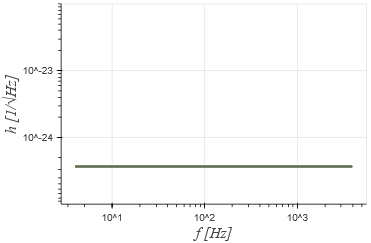
\includegraphics[width=0.5\textwidth]{SPQ_aLIGO_residualgas.png}
    \caption{The residual gas noise model is a limiting `floor' to the
      noise model. It is not frequency-dependent, so appears as a
      straight line across the graph.}
    \label{fig:residual}
    \end{figure}
    The residual gas pressure influences the refraction index of the inner interferometer arms, 
    \[
    n = 1 + \epsilon\frac{\mathcal{P}_{arm}}{\mathcal{P}},
    \]
    where $\epsilon \approx 1.2\times 10 6{-4}$ \cite{VIRGO}, and
    $\mathcal{P}$ is the atmospheric pressure in mbar. The VIRGO
    design document gives the strain due to radiation pressure
    fluctuation as
    \[
    h_{RG} = \frac{\epsilon\pi^{\frac{1}{4}}}{N_{atmos}}\sqrt{\frac{w_{beam}N_{arm}}{v_{H2}V_{beam}}} \approx 2.5 \times 10^{-26},
    \]
    where $w_{beam}$ is the beam waist far from the mirror ($\sim
    0.1m$), $v_{H2}$ is the molecular velocity, $V_{beam} = \pi
    w_{beam}^2L_{arm}$ is the `beam volume', and $N_{arm}$ and
    $N_{atmos}$ are the molecular densities in the arm and in the
    atmosphere, respectively.
    The arm pressure, $P_{arm}$, is calculated in units of mbar as
    \begin{equation}
    \label{eq:pressure}
    \mathcal{P}_{arm} = \mathcal{P}e^{-8N_p} + 10e^{-4N_p} + 10^{-3}e^{-2N_p} + 10^{-8}{-0.7N_p} + 10^{-11}e^{-0.3N_p} + 10^{-16}.
    \end{equation}
   This is an approximation of the sum of partial pressures of the
   main gasses contributing to the residual gas. The final component
   of this calculation is the only part that is independent of the
   number of vacuum pumps, $N_p$. It is thus the minimum pressure that
   a user can reach.
    The equation used to calculate the strain due to residual gas
    pressure fluctuations is then
    \begin{equation}
        \label{eqn::residual} 
        h_{RG} = 1.37 \times 10^{-18} \times \sqrt{\frac{\mathcal{P}_{arm}}{L}}.
    \end{equation}
    \item \textbf{Quantum Noise} \\
    \begin{figure}[h!]
    \centering
    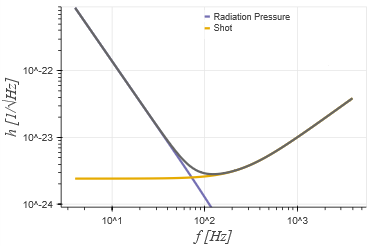
\includegraphics[width=0.5\textwidth]{SPQ_aLIGO_quantum.png}
    \caption{The quantum limit in Space Py Quest, formed by the combination of radiation pressure noise and shot noise.}
    \label{fig:quantum}
    \end{figure}
    \begin{itemize}
        \item \textbf{Radiation Pressure} \\
    The radiation pressure noise calculation in Space Py Quest is an
    adaption of equation (12) in \cite{VIRGO}, 
    \[
    h_{RP} = \frac{16\sqrt{2}\mathcal{F}}{LM(2\pi f)^2}\sqrt{\frac{hF_{PR}P}{4\pi^2c\lambda}}\sqrt{\frac{1}{1 + \left(\frac{f}{f_{FP}}\right)^2}}.
    \]
    In this expression, $\mathcal{F}$ is the arm cavity finesse,
    $F_{PR}$ is the power recycling factor, $c$ is the speed of light,
    $\lambda$ is the wavelength of the laser light, and $f_{FP}$ is
    the Fabry-Perot cut-off frequency, defined as
    \begin{equation}
        f_{FP} = \frac{c}{4L\mathcal{F}}.
    \end{equation}
    We make the simplification
    \[
    \sqrt{8} = 2\sqrt{2} = \frac{16 \sqrt{2}}{8} = \frac{16 \sqrt{2}}{(2)^2 \times \sqrt{4}}
    \]
   and multiply the result by the square root of the product of the
   mirror material damping rate $\mathcal{L}$ and the mirror surface
   roughness loss $\mathcal{L}_R$,
   $\sqrt{\mathcal{L}\mathcal{L}_R}$. The power scaling of these
   values is again arbitrary. The radiation pressure noise is then
    \begin{equation}
    \label{eqn::radiation}
    h_{RP} = \frac{\mathcal{F}}{LM\pi^3f^2}\sqrt{\frac{8hF_{PR}P}{c\lambda}}\sqrt{\frac{1}{1 + \left(\frac{f}{f_{FP}}\right)^2}} \times \sqrt{\mathcal{L}\mathcal{L}_R}.
    \end{equation}
  
    \item \textbf{Shot} \\
    Shot noise is given in equation (11) of \cite{VIRGO} as
    \begin{equation}
    h_{Sh} = \frac{1}{8L\mathcal{F}}\times\sqrt{2h\frac{\lambda c}{\eta F_{PR}P}}\times\sqrt{1 + \left(\frac{f}{f_{FP}}\right)^2}.
    \end{equation}
    In Space Py Quest, we assume that the photodetector efficiency
    $\eta$ is 100\%, such that $\eta = 1$. We also include the
    lossiness due to the roughness of the surface, so that the noise
    calculation used is
    \begin{equation}
    \label{eqn::shot}
    h_{Sh} = \frac{1}{8L\mathcal{F}}\times\sqrt{2h\frac{\lambda c}{F_{PR}P}}\times\sqrt{1 + \left(\frac{f}{f_{FP}}\right)^2}\times\mathcal{L}^{-\frac{1}{2}}\mathcal{L}_R^{-5}.
    \end{equation}
    The powers to which $\mathcal{L}$ and $\mathcal{L}_R$ are raised are arbitrary.
    \end{itemize}
\end{itemize}

%\clearpage
\section{Making Space Py Quest}
\label{sec:making}
\subsection{Code Structure}
\label{sec::structure}
\begin{figure}[h!]
    \centering
    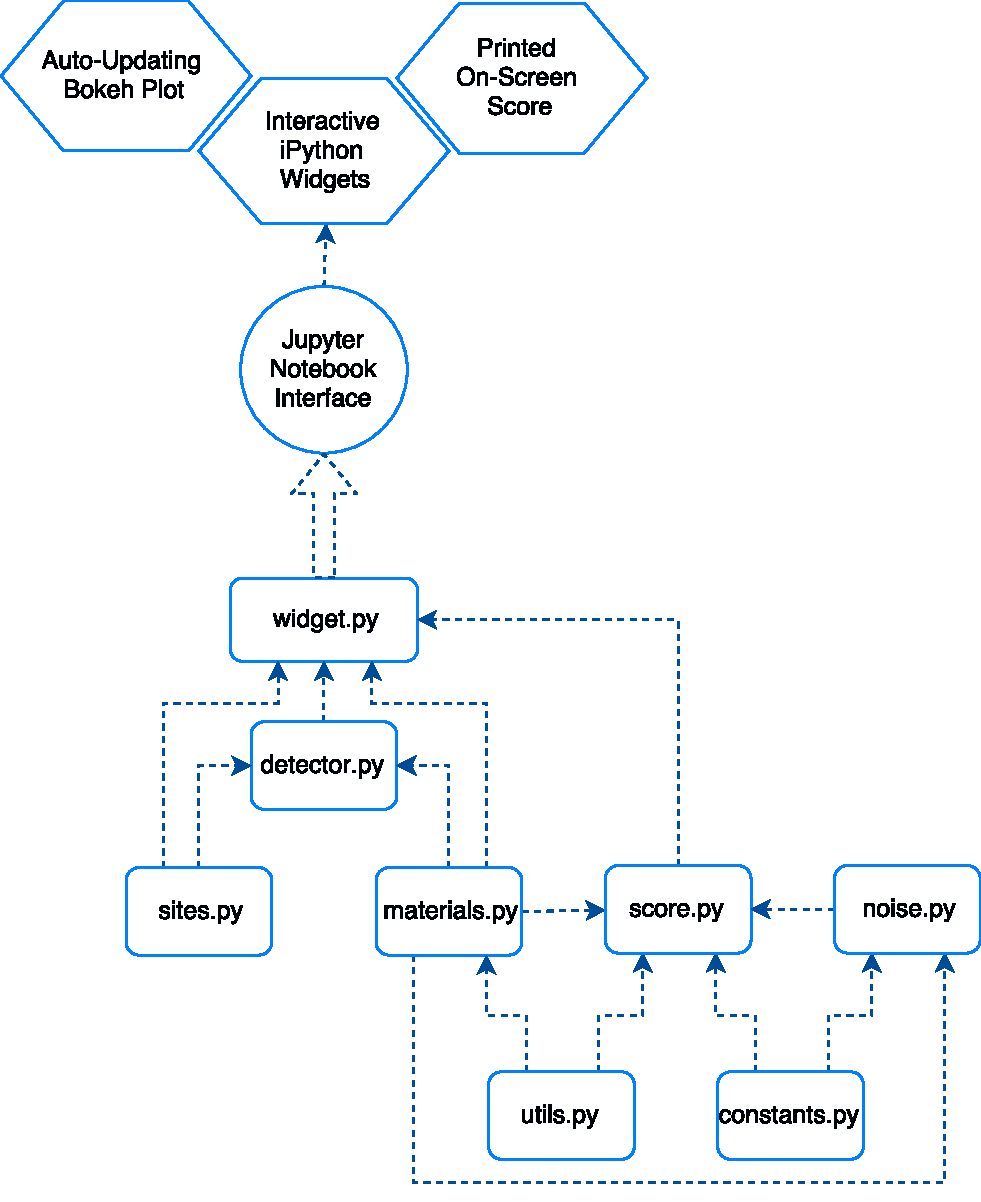
\includegraphics[scale=0.75]{SPQstructure.pdf}
    \caption{Code structure diagram for Space Py Quest. Utility
      functions and constants, defined in the appendices of this
      document, are held in $utils.py$ and $constants.py$
      respectively. These are used throughout the rest of the game
      code. All other $.py$ files displayed define the game
      classes. The \textbf{Detector} class is defined in
      $detector.py$. This imports $sites.py$ and $materials.py$ so
      that it can initialise its own location and mirror material
      parameters if the user does not provide them. The game interface
      is managed by the \textbf{spaceTimeQuest} class, which both
      handles the interaction of the iPython widgets with the Bokeh.io
      plot, and the interaction of the \textbf{Score} class with the
      detector object. \textbf{Score} and \textbf{ScoreCalculator} are
      defined in $score.py$, which calculate the figures of merit for
      the detector they are passed. They utilise all of the noise
      classes defined in $noise.py$ to generate and return the
      detector's noise curves, cost, complexity, range, and the number
      of detections of different types of event.}
    \label{fig:spq1}
\end{figure}
\begin{figure}[h!]
    \centering
    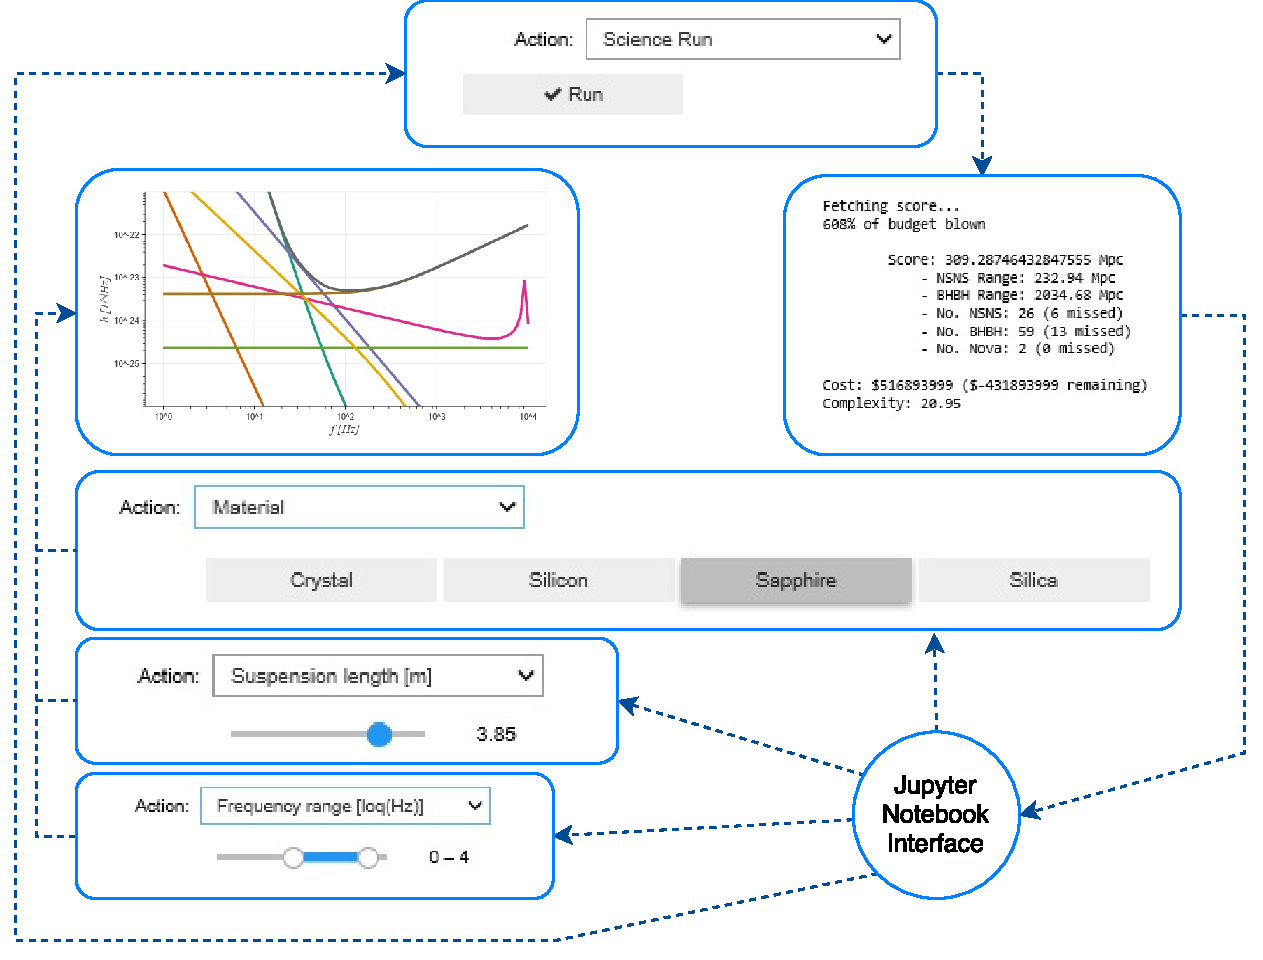
\includegraphics[scale=0.75]{close-up.pdf}
    \caption{Illustration of some available widget types and the
      interactive output, both existing within the Jupyter Notebook
      interface. The categorical variables of location and mirror
      material are changed using toggle buttons. Continuous variables,
      like suspension length and mirror surface roughness, are altered
      using float-type slides. Discrete variables like the number of
      suspension stages are incremented using similar, integer-type
      sliders. The ranges displayed on both axes are varied using
      float-type range sliders. There are also tick boxes - not
      illustrated - which allow the user to determine which noise
      curves are displayed. The score calculation and display is
      triggered by a press of the $Run$ button, which represents the
      detector activating a `Science run'.}
    \label{fig:spq2}
\end{figure}

%\clearpage
Space Py Quest is written in Python. The driving code has a
semi-object-oriented structure, as illustrated and described in figure
\ref{fig:spq1}. The interactive elements of the game, existing in the
Jupyter Notebook, are enabled using iPython Widgets, with a Bokeh.io
plotting mechanism. iPython Widget examples are shown and described in
figure \ref{fig:spq2}. In addition to these, there are also Tick Boxes
that determine which noise curves are shown. Each widget responds to
user interaction, triggering recalculation of the noise curves and
updating the displayed plot accordingly. The fraction spent of the
user's budget is also continuously updated as the detector parameters
change.

\textbf{Suggestions for Structure Modifications}\\
As shown in figure \ref{fig:spq1}, the $materials$ and $sites$ classes
must be imported by both $detector$ and $widget$. This is because
$widget$ must know about these classes in order to set detector
values, and $detector$ must know about them in order to initialise
itself with values, if none are provided by the user. Space Py Quest
was designed to be adaptable to detectors that might have different
sites or materials, but this is not necessarily a useful feature.  It
is proposed that instead, all parameter ranges and class names are
stored in $constants$, and passed through $detector$ to
$widget$. Alternatively they could be passed straight to $widget$,
without the option for the detector to initialise its own values. 

% [IRS:RV do you think this needs a reference?]
\begin{comment}
\begin{itemize}
    \item Detector\\
    Space Py Quest's $detector$ class has been heavily modified from
    its initial translation from Space Time Quest. It now holds 5
    dictionaries as its only data members, allowing its contents to be
    modified by users without requiring them to change the class
    itself. In its initial form, the dictionaries hold the following
    values.
    \begin{itemize}
        \item $names$ \\
        \begin{itemize}
            \item $['freqrange'] =$ `Frequency range [loq(Hz)]'
            \item $['site'] =$ `Location'
            \item $['depth'] =$ `Depth [m]'
            \item $['pumps'] =$ `No. vacuum pumps'
            \item $['temperature'] =$ `Temperature [K]'
            \item $['sus\_stages'] =$ `No. suspension stages'
            \item $['sus\_length'] =$ `Suspension length [m]'
            \item $['mirror\_mass'] =$ `Mirror mass [kg]'
            \item $['power'] = $`Laser power [W]'
            \item $['material'] =$ `Material'
            \item $['roughness'] =$ `Roughness [nm]'
        \end{itemize}
        $names$ gives the names that are printed to the on-screen drop
        menu for the Space Py Quest interface. The parameters they
        refer are held in the $parameters$ dictionary.
        \item $parameters$ \\
        \begin{itemize}
            \item $['freqrange'] \rightarrow$ Frequency range, $\mathbf{f}$ (Hz), initialised to $f \in (10^0, 10^4)$ Hz
            \item $['site'] \rightarrow$ Detector site, initialised to $Jungle$
            \item $['depth'] \rightarrow$ Underground depth of the detector, $d$ (m), initialised randomly
            \item $['pumps'] \rightarrow$ Number of vacuum pumps per kilometer, $N_p$, initialised randomly
            \item $['temperature'] \rightarrow$ Temperature of the detector, $T$ (K), initialised randomly
            \item $['sus\_stages'] \rightarrow$ Number of suspension stages, $N_s$, initialised randomly
            \item $['sus\_length'] \rightarrow$ Length of suspension, $l$ (m), initialised randomly
            \item $['mirror\_mass'] \rightarrow$ Mirror mass, $M$ (kg), initialised randomly
            \item $['power'] \rightarrow$ Laser power, $P$ (W), initialised randomly
            \item $['material'] \rightarrow$ Mirror material, initialised to $Silicon$
            \item $['roughness'] \rightarrow$ Surface roughness, $R$ (nm), initialised randomly
        \end{itemize}
        % SORRY
        \item $options$\\
        Both $materials$ and $sites$ must have string identifiers for
        each class defined for ease of display in the Jupyter
        notebook. These are just the class names, so the dictionary
        holds just two arrays containing strings:
        \begin{itemize}
            \item $['material'] = ['Crystal', 'Silicon', 'Sapphire', 'Silica']$
            \item $['site'] = ['City', 'Jungle', 'Desert', 'Island']$
        \end{itemize}
   
    \item Sites\\
    
    \item Materials\\
     Each material class defines the same two functions, $GetQ$ and
     $GetCost$. In MAGIC all calculations shared by subclasses of the
     same type are declared first in a parent class. $GetCost$ returns
     the cost $\mathcal{C}$,

    \begin{equation}
        \mathcal{C} = C_0 + A_0\left(\frac{M}{100}\right)^2,
    \end{equation}
    and $GetQ$ returns the mechanical quality factor, $\mathcal{Q}$,
    \begin{equation}
        \mathcal{Q} = \frac{1}{\mathcal{I}(\mathbf{T}(x), \mathbf{q}(T(x)), T)}.
    \end{equation}
    Here, $\mathcal{I}$ is the interpolation function given in
    equation \ref{eq:lerp}, T is the temperature of the detector, and
    $\mathbf{q}(T)$ is an array of mirror losses related to
    temperature array $\mathbf{T}$. $\mathbf{q}(T)$ and $\mathbf{T}$
    are defined for each material as given below.
    \begin{itemize}
        \item Sapphire \\
        \[ \mathbf{T}(x) = [1, 25, 80, 105, 230, 300 ] K
        \]
        \begin{equation}
        \label{eqn::qsapp}
            \mathbf{q}(T) = [1.4e-9, 2.5e-8, 7e-9, 1.2e-8, 1.6e-8, 1e-7 ].
        \end{equation} 
        \item Crystal \\
        \[ \mathbf{T}(x) = [1, 300 ] K
        \]
        \begin{equation}
        \label{eqn::qcrys}
        \mathbf{q}(T) = [1e-3, 1e-3 ].
        \end{equation}
        \item Silicon \\
        \[ \mathbf{T}(x) = [1, 32, 40, 270, 300 ] K
        \]
        \begin{equation}
        \label{eqn::qsilicon}
             \mathbf{q}(T) = [1.4e-9, 1.5e-8, 7.5e-9, 4.5e-8, 7e-8 ].
        \end{equation}
        \item Silica \\
        \[ \mathbf{T}(x) = [1, 35, 90, 150, 200, 250, 300 ] K
        \]
        \begin{equation}
        \label{eqn::qsilica}
            \mathbf{q}(T) = [1e-3, 7e-4, 1e-4, 3e-6, 3e-7, 1.5e-7, 1.5e-7 ].
        \end{equation} 
    \end{itemize}
    
    The $materials$ file also defines a $GetRoughnessLoss$ function,
    which returns the loss, $\mathcal{L}_R$, due to the mirror surface
    roughness $R$,
    \begin{equation}
        \mathcal{L}_R = 1 + \frac{0.9}{499}(1 - R) .
    \end{equation}
    \item Score \\
    The $score$ data members, listed below, are all set to 0 at instantiation.
    \begin{itemize}
        \item $N_{bhbh} \rightarrow$ Number of black hole binaries detected
        \item $N_{nsns} \rightarrow$ Number of neutron star binaries detected
        \item $N_{sn} \rightarrow$ Number of supernovae detected
        \item $r_{bhbh} \rightarrow$ Range within which binary black holes can be detected
        \item $r_{nsns} \rightarrow$ Range within which binary neutron stars can be detected
    \end{itemize}
    A $Score$ object is set up by a $ScoreCalculator$, which changes these values.
    \item Score Calculator\\
    The data members of the score calculator include a $Detector$, the
    minimum and maximum frequency ($f_{lo}$ and $f_{hi}$) of the
    detector range to investigate, and the number of data points,
    $N_{data}$, to plot. There are also two dictionaries:
    $noiseModels$, which holds noise objects, and $noisesUsed$, which
    uses the same keys to dictate whether or not the stored noise
    models are actually taken into account in the calculation. This
    was added to test adaptability to detectors that may not
    experience noise that other detectors do. For example, space-based
    interferometers would not experience seismic noise. Noise models
    that correspond to a key for whom $noisesUsed$ is set to $False$
    are not taken into account in the final score calculation, and are
    not shown in the plot.  
    \item Noise \\
    Each $...Noise$ model declares one static method, $Get...Noise$,
    and one class method, $ComputePoint$. The latter simply returns
    the output of the former, but with a overarching naming convention
    that allows this function to be called for any unknown noise
    model. Static methods cannot alter class or object state, whilst
    class methods cannot alter object state. This idea has been
    utilised in MAGIC, where noise models $must$ have one externally
    accessible function that returns its noise curve, the name of
    which is identical to that providing the noise from each other
    noise model.
\end{itemize}
\end{comment}
%This was re-thought in MAGIC, where the noise models calculate the whole noise curve for a frequency array $\mathbf{f}$ in a single function

%\begin{comment}
\subsection{Changes to Arbitrary Factors (Section for Internal Copy Only)}
\label{sec:changes}
Having an open-source Python version of the Space Time Quest giving
\textit{exactly} the same results would provide a handy tool for
finding the best score. To avoid Space Py Quest facilitating dishonest
corruption of the leaderboard, certain constant factors were altered
in the translation to Space Py Quest. These changes are encapsulated
in the table below.
\begin{center}
    \begin{tabular}{ |c|c|c|c|c| } 
     \hline
     \textbf{Name (if given)} & set in & \textbf{Symbol}  & \textbf{STQ}  & \textbf{SPQ}  \\ 
     \hline
     \textbf{High frequency floor} & \textit{sites.py}  & $X_{hf}$ &  &\\
     City & & & $8 \times 10^{-12}$ & $1 \times 10^{-11}$ \\
     Jungle & & & $2 \times 10^{-14}$ & $5 \times 10^{-14}$ \\
     Desert & & & $1 \times 10^{-14}$ & $8 \times 10^{-15}$ \\
     Island & & & $2 \times 10^{-12}$ & $9 \times 10^{-13}$ \\
     \hline
       & $noise.py \rightarrow MirrorThermalNoise $ & $A_{MT}$ & 25000 & 20505\\ 
     \hline
     \textbf{Cooling cost ($C_{temp}$) constants} & $score.py \rightarrow CalcCost$  & & &  \\ 
     if $T > T_N$ & & $A_{T, 1}$ & 20000 & 20102 \\
     else & & $A_{T, 2}$ & 10000 & 10201 \\
     \hline
     \textbf{Vibration cost ($C_{vib}$) constants}  & $score.py \rightarrow CalcCost$  &  &   & \\ 
     &  & $a_v$  &  1.7 & 2.1 \\
     &  & $c_v$  &  1.5 & 1.2 \\
     \hline
    \end{tabular}
    \label{tab:changes}
    \end{center}
%\end{comment}
\begin{comment}
\section{Making Space Pie Quest}
\begin{figure}[h]
    \centering
    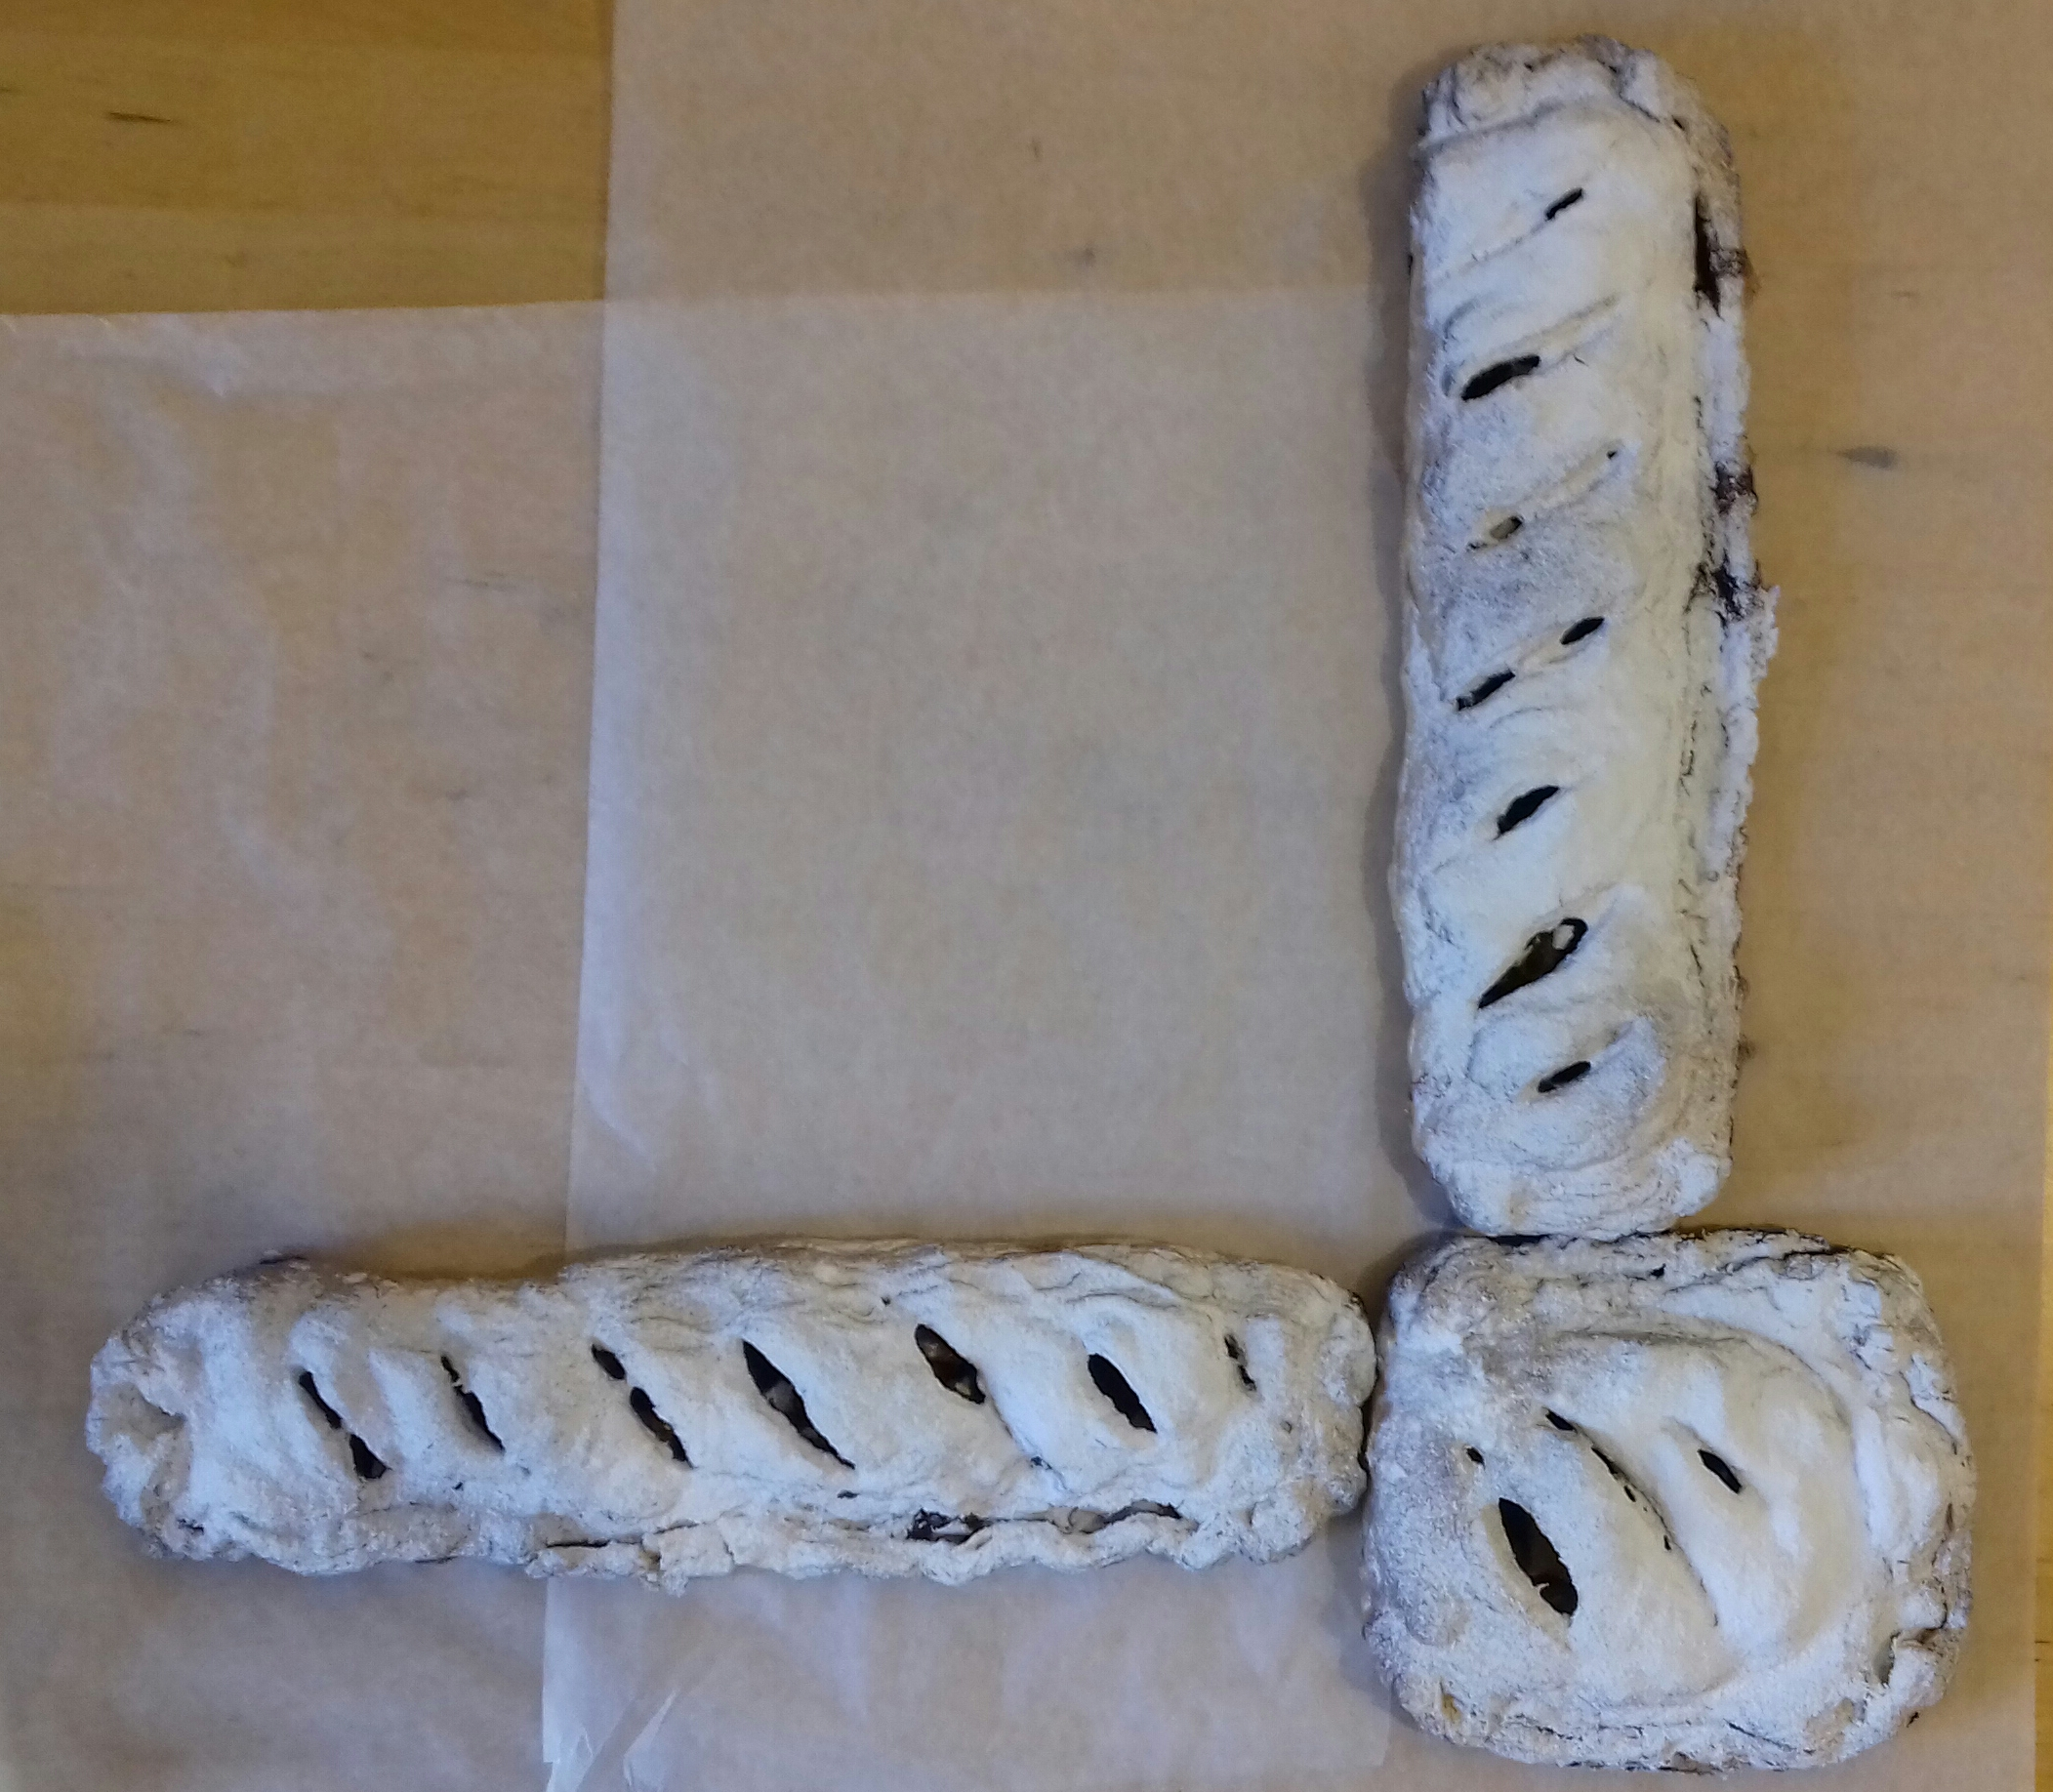
\includegraphics[scale=0.05]{PieGO.jpg}
    \caption{The finished product, PieGO.}
    \label{fig:PieGO}
\end{figure}
Space Pie Quest, or PieGO, is an interferometer made of
pie. Specifically, apple strudel pie. It's made with ALDI ingredients,
so it's cheap, and it's also vegan, and delicious. Thus, we maximise
taste whilst minimising harmful consequences to the planet and our
pockets.  

\subsection{Translation from non-vegan recipe}
This pie is based on a recipe found here:\\
\url{http://allrecipes.co.uk/recipe/16001/quick-apple-strudel.aspx}. This
uses an egg for glazing, which we replace with soy milk. 

\subsection{Pie Structure}
First make your pie. Follow the instructions in the link given, and
ensure that you make 2 long rectangular pies and 1 square one. At the
assembly stage, wait until pies have cooled until configuring into a
big `L' shape with the square at the vertex. Congratulations; you have
an interferometer-shaped pie. Dust this with icing sugar and serve.

\subsection{Implementation}
Eat, or enter (and win) a competition for `best physics-themed bake'.
\end{comment}

%\clearpage
\section{Testing Space Py Quest}
\label{sec:testing}
In order to ensure that Space Py Quest performs as expected, checks
were completed before release. These included comparison to the
original Space Time Quest game and realistic sensitivity curves for
aLIGO, as well as confirming that the individual noise curves scaled
as expected. The maximum number of detections were found to ensure
that the optimal parameters in the game correspond to realistic
expectations. Finally, detections of different sources in selected
frequency bands were examined, in order to verify that greater
sensitivity at high frequency outputs more neutron star binary
detections.  
\label{sec:mcmc}

\subsection{Comparison to Space Time Quest}
%Space Time Quest was released in 2017 and has an online leaderboard, where a maximum number of 281 detections has been achieved. This can be used as threshold when attempting to find the high score: the MCMC has to return a score at or above this value. Therefore, the MCMC was first used to obtain the high score for this game, in order to ensure that it performs as expected. Then it would be used to find the high score for Space Py Quest, which does not currently have a leaderboard or as many users to give an indication of the highest score achievable.

The original version of Space Py Quest ported to Python (before the
arbitrary scaling factors were added) was compared to the released
version of Space Time Quest. During this comparison, it was found that
Space Time Quest did not include the suspension thermal noise when
calculating the total noise and therefore the maximum detector
range. Therefore, the suspension thermal noise was taken out of
Space Py Quest when calculating the score, for a full comparison.

It was found that detector depth behaved differently in the two
versions, despite the code being identical. Both games returned the
same maximum number of detections, 281. The difference was very
slight, meaning that with all parameters set to optimal values, the
depth would need to be over 12m to achieve 281 detections in the C\#
version, whereas this was possible for any value from 0 to 20m in the
Python version. This was concluded to be due to different rounding
errors present in the two languages. 

As mentioned in section \ref{sec::differences}, the different
integration technique used for the distance calculation also lead to
slight discrepancies, but has considerably helped speed up the Markov
chain Monte Carlo (MCMC) algorithms used to find the high scores. The
MCMC currently iterates over multiple chains for around 10$^6$ points
to output the high score, and each run takes around 30
minutes. Therefore, the original integration method would have been
unreasonably slow. Other than these two changes, no differences
between the two versions of the same game have been found, suggesting
that Space Py Quest should work as expected.

\subsection{Testing Validity of Individual Noise Curves}
The noise curves displayed by the Space Py Quest plotting interface
were individually tested to ensure that they correspond accurately to
their respective noise equations. This included examining the scaling
of the curves with relevant. The scalings are considered in terms of
the conventional log-log plot for detector sensitivity curves, and are
outlined below. In addition, sensitivity values at arbitrary
frequencies were evaluated, and can be seen in table
\ref{tab::checks}.

%, albeit with the inclusion of the scaling factors to ensure that it is different to the original game. It also contains extra features to make it more enjoyable, e.g. inclusion of the detection of a supernovae for a good mid-high frequency range sensitivity. While this is not entirely realistic, it adds another goal for the user to achieve and can also aid in the teaching of different gravitational wave sources. 

As Space Py Quest is in essence a simplified gravitational wave
detector sensitivity modelling software, the scaling of the noise
curves can be compared to those produced by the more realistic
\textit{Gravitational-Wave Interferometer Noise Calculator}
(GWINC)\cite{GWINC}. Parameters that approximately matched up to the
aLIGO detector were input into Space Py Quest. These parameters were
found using the aLIGO model used in GWINC, and consisted of $d=0$m,
$N_p=6$, $N_s=4$, $l=0.6$m, $M =40$kg, $P=125$W, $r=1$nm, $T=295K$ and
mirror material of Silica. The detector arm length, which is typically
constant in the game, was set to 4000m to mirror aLIGO. 

The aLIGO location is not an option is Space Py Quest, so the location
that appeared to have the most similar values for seismic and gravity
gradient noise (Island) was selected. Noise curves produced with these
parameters and the aLIGO model in GWINC are shown in figure
\ref{fig::SPQGWINCaLIGO}. 

 \begin{figure}[h!]
     \centering
         \begin{subfigure}{\textwidth}
        \centering
         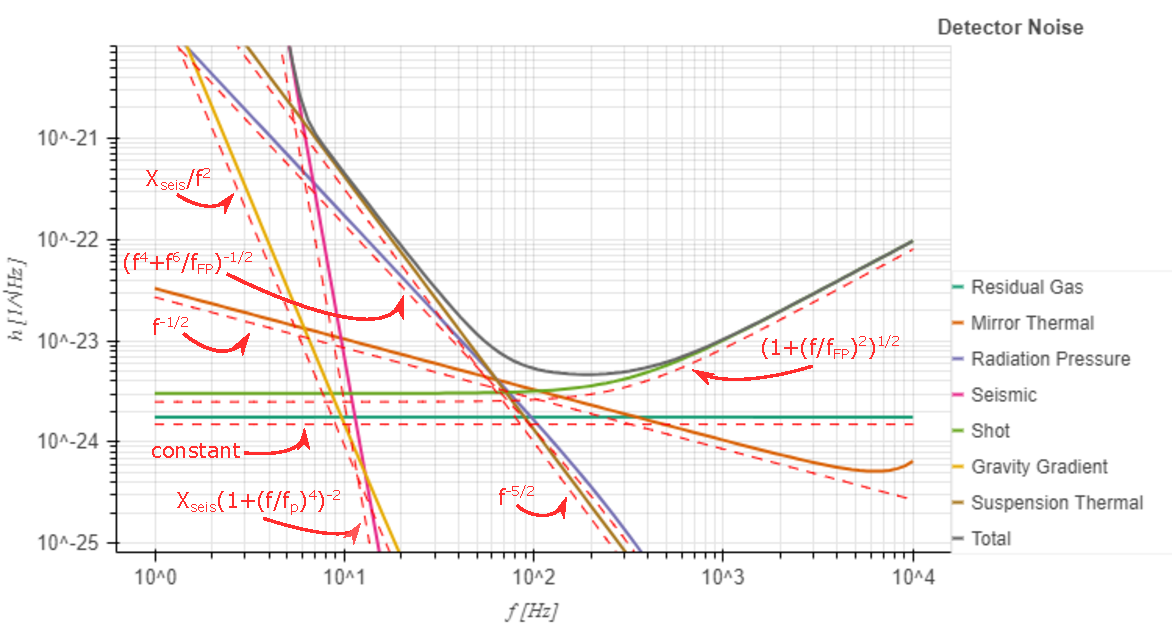
\includegraphics[width=0.9\textwidth, trim = {0 0 0 0.7cm}, clip]{SPQaLIGOscalings.pdf}
         \caption{Noise curves produced by Space Py Quest for aLIGO model}
         \label{fig::PowerStages}
         \end{subfigure}%\hfill 
         \\
        \begin{subfigure}{\textwidth}
        \centering
         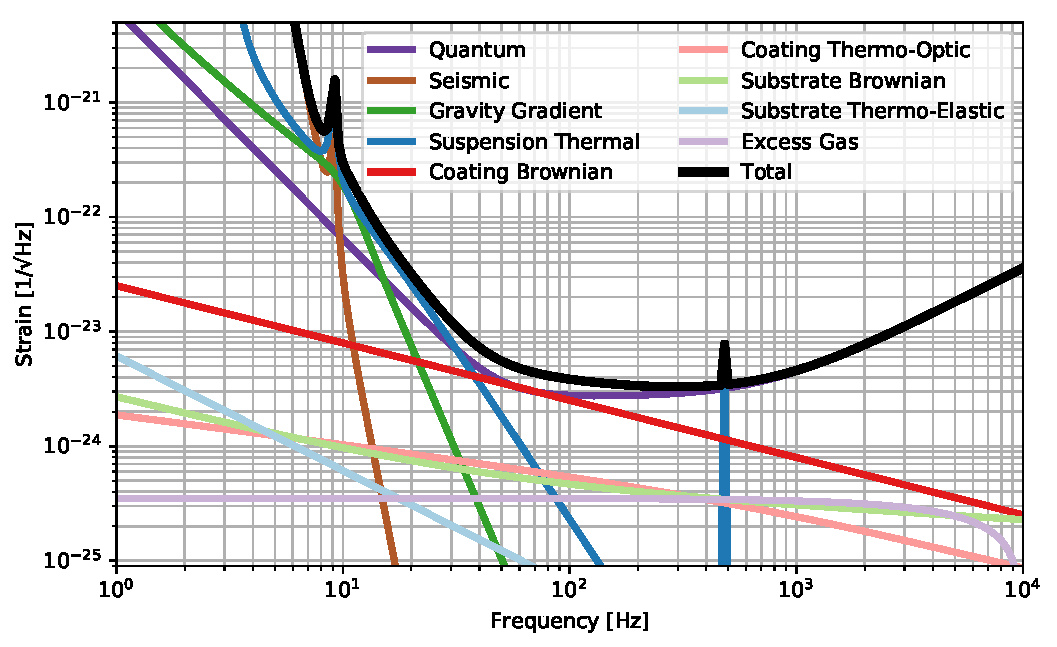
\includegraphics[width=0.73\textwidth, viewport=50 0 560 310]{gwinc_aLIGO.pdf}
         \caption{Realistic noise curves produced by GWINC for aLIGO model}
         \label{fig::PowerStagesMass}
         \end{subfigure}
         \caption{Noise curves for aLIGO model produced by Space Py
           Quest and GWINC. The maximum sensitivity for both appears
           to be around the same value, and both curves are mostly
           limited by seismic, suspension thermal and quantum shot
           noise.}
         \label{fig::SPQGWINCaLIGO}
 \end{figure}

The quantum noise in GWINC includes both radiation pressure and shot
noise, whereas the coating and substrate noises are combined into
mirror thermal noise in Space Py Quest. As an overview, it can clearly
be seen that total noise curves follows a similar shape, with minimum
strain between 10$^{-23}$Hz$^{-1/2}$ and 10$^{-24}$Hz$^{-1/2}$. They
both appear to be mostly limited by shot noise and suspension thermal
noise, with seismic noise dominating at low frequencies. An obvious
difference between the two is the greater number of spikes due to
resonant modes included in GWINC. This difference is assumed to be due
to the simplified equations used in the game. The scalings for
individual noise curves are detailed below. 

\begin{enumerate}
    \item \textbf{Residual Gas Noise} \begin{itemize}
    \item Frequency: Residual gas noise is the only noise that does
      not depend on frequency, and therefore is a horizontal line in
      the sensitivity plot at any parameter values. In the GWINC plot,
      however, this noise decreases at higher frequency, suggesting
      that a more realistic implementation of residual gas would have
      this effect. 
    \item Number of pumps: The dependence on this parameter can be
      seen in equation \ref{eqn::residual}. This equation suggests
      that although the addition of pumps lowers noise, this effect
      should decrease as $N_p$ increases, which can be seen by
      altering this variable in Space Py Quest. The number of pumps
      was set to six to replicate the GWINC aLIGO model, but this
      appears to produce a higher value of noise. This is attributed
      to the simplification of residual gas used in the game.  
   \end{itemize}
    
    \item \textbf{Mirror Thermal Noise}
    \begin{itemize}
    \item Frequency: This noise curve declines over frequency in the
      game, which can be explained by the $\omega^{-1/2}$ dependence
      in equation \ref{eqn::mirror}. At higher frequencies, the
      resonance in the $(\omega_1^2-\omega^2)^{-1/2}$ term leads to a
      spike at the resonant frequency of the mirror. This can be seen
      more clearly in figure \label{fig::SPQMaxNoLim}. The coating and
      substrate noises in GWINC are combined into the mirror thermal
      noise function, and it can be seen that the dominant coating
      Brownian noise follows a similar scaling and value to those
      produced by Space Py Quest, omitting the resonance. The
      resonance in the game is partially arbitrary. 
    \item Mirror mass: The mass dependency in mirror thermal noise can
      be seen in the $M_{eff}$ and $\omega_1$ terms in equation
      \ref{eqn::mirror}. The first term suggests that increasing mass
      increases noise. However, the mass dependence in the second term
      means that as mass increases, noise increases, and appears to
      dominate. It also describes the resonant frequencies of the
      mirror, which decreases as mirror mass increases. This behaviour
      can be seen when varying the parameters in the game.
    \item Mirror material quality and temperature: The noise is
      proportional to $\sqrt{T}$, so as $T$ increases the noise should
      increase. However, the optical loss dependence on temperature
      (described in appendix \ref{app::material}) appears to dominate,
      meaning that after around 30K the noise curve decreases until
      approximately 250K, where it starts to increase in noise again. 
	\end{itemize}
    
    \item \textbf{Radiation Pressure Noise}
    \begin{itemize}
    \item Frequency: This noise is proportional to
      $(f^4+f^6/f_{FP})^{-1/2}$ as shown in equation
      \ref{eqn::radiation}, and the effect of the noise decreasing
      with frequency can be seen in Space Py Quest. In GWINC,
      radiation pressure is the dominant quantum noise at low
      frequencies, which appears to follow a similar scaling.  
\item Power and mirror mass: It is also proportional to $P^{1/2}$ and
  $M^{-1}$, and both responses can again be seen when altering the
  respective parameters in the game.
\item Mirror material loss: Radiation pressure noise depends on the
  mirror material damping factor as $\mathcal{L}^{1/2}$. All material
  losses are identical except for Crystal, which is more lossy than
  the other materials and therefore has a smaller value of
  $\mathcal{L}$. This is depicted by a constant decrease in the
  radiation pressure noise across all frequencies when Crystal is
  selected in the game. Swapping between the other materials has no
  effect on this noise, as expected.
\end{itemize}
    %more loss, less power, less rad pressure. 
    
    \item \textbf{Seismic Noise}
    \begin{itemize}
    \item Frequency, number of stages and location: The frequency
      dependence of seismic noise is encompassed in the
      $\mathcal{T}_{pend}$ and $X_{seis}$ terms in equation
      \ref{eqn::seismic}, and is also dependent on the number of
      stages and location. Keeping the latter two constant, the
      $(f/f_p)^2$ value in $\mathcal{T}_{pend}$ term prevails at low
      frequency, meaning that noise is initially constant and then
      decreases with frequency. When the left and right hand sides of
      the $\mathcal{T}_{pend}$ denominator tend towards the same
      value, a resonance peak can be seen. At greater frequencies, the
      $(f/f_p)^4$ term dominates, meaning that noise again decreases
      with frequency. These frequencies dependencies are all
      multiplied by the $1+(f/f_c)^{n_0}$ in $X_{seis}$, which too
      becomes less dominant at greater frequencies. All these effects
      can be seen in Space Py Quest, with the initial decrease in
      frequency being affected by changing location, and the resonance
      becoming more peaked at a greater number of stages. The number
      of stages is an exponent, so altering it should change the
      gradient of the line, which appears to be the case in the
      game. The seismic resonance can be seen at higher frequencies in
      GWINC, after which it follows a similar scaling to that in
      Space Py Quest. 
    \item Suspension length: The suspension length dependency is
      similar to the frequency dependence in $\mathcal{T}_{pend}$,
      except with $f\rightarrow l^{1/2}$, which makes the distribution
      wider. Increasing the suspension length increases noise at very
      low frequencies but decreases it at values of 1Hz and higher,
      when the $X_{seis}(f/f_p)^4$ term is again dominant. 
    \item Depth: The final parameter that affects seismic noise is
      depth. It is proportional to $(1+\frac{d}{50}^4)^{-1/2}$,
      meaning that above 50m, noise decreases with depth. Similar to
      suspension length, the effect is smaller at larger depths. Below
      50m, an increase in digging does not change the noise curve by a
      significant amount. This was confirmed by the Space Py Quest
      interactive plot.
    \end{itemize}
    
    \item \textbf{Shot Noise}
    \begin{itemize}
    \item Frequency: The frequency dependence of this noise is
      $(1+\left(\frac{f}{f_{FP}}\right)^2)^{1/2}$, meaning that noise
      increases with frequency. This can be seen in Space Py Quest,
      where the noise appears constant until the frequency becomes the
      dominant term and the noise increases linearly with
      frequency. The shot noise is the dominant quantum noise at
      higher frequencies in GWINC, and again follows a similar scaling
      to the game. 
    \item Roughness: The roughness dependence is
      $(1+(0.9/499)(1-R))^{-5/2}$, meaning that as roughness
      increases, shot noise increases, with greater effect at greater
      roughness. 
    \item Power and mirror material loss: This noise is depends on
      power and mirror material damping factor according to $P^{-1/2}$
      and $\mathcal{L}^{-1/2}$, meaning that an increase in either of
      these parameters decreases shot noise.
    \end{itemize}
    
    \item \textbf{Gravity Gradient}
    \begin{itemize}
    \item Frequency: The frequency dependence of this noise is
      $X_{seis}(f)/f^2$ , and can be seen as a line of negative
      gradient in Space Py Quest. At higher frequencies, the $1/f^2$
      becomes more dominant, and this transition can be seen as a
      `knee' in the game. In GWINC, the more realistic gravity
      gradient noise leads to a different scaling at lower
      frequencies, until it transitions into a scaling that appears
      similar to Space Py Quest. 
    \item Location and depth: It is also dependent on location and
      depth, and this relation is identical to that in seismic
      noise. Therefore, the same effect can be seen when altering
      these parameters. 
    \end{itemize}
    
    \item \textbf{Suspension Thermal}
    \begin{itemize}
   \item Frequency: Suspension thermal has a frequency dependence
     $f^{-5/2}$, which is a power law and therefore is displayed as a
     straight line decreasing in value in Space Py Quest. Ignoring the
     realistic resonances included by GWINC, this noise curve again
     appears to follow a similar scaling to the game. 
   \item Mirror mass and suspension length: As the mass dependence is
     $M^{-1/4}$, the noise decreases with increasing mass, with the
     effect decreasing at greater mass. The noise also scales with
     suspension length as $l^{-1}$, which produces a similar effect to
     varying mass, but with a greater gradient. 
   \item Temperature: The suspension thermal noise is proportional to
     $\sqrt{T}$, so increases with temperature. 
 \end{itemize}
\end{enumerate}
Check for varying detector configuations for each noise curves can be
seen in table \ref{tab::checks}. All parameters are set to mirror the
aLIGO model at the initiation of each check, and the original values
were multiplied by the relevant scaling factors to ensure that they
returned identical results to the noise calculations and the
interactive plot in Space Py Quest. 

     \begin{table}[h]
     \centering
     \captionsetup{width=0.9\textwidth}
      \caption{Point checks for individual noise curves. The new
        strain obtained when altering selected parameters at varying
        frequencies is shown. The values obtained correspond to what
        can be seen in the Space Py when setting these parameters, and
        also what is output by multiplication by the relevant scaling
        factors, confirming how the plot and calculations are as
        expected.}
      \label{tab::checks}
    \begin{tabular}{ |c|c|c|c|c| }
     \hline
     \textbf{Noise} & \textbf{Frequency [Hz]} & \textbf{aLIGO} $h$ [Hz$^{-1/2}$] &\textbf{Altered Parameters}    & \textbf{New} $h$ [Hz$^{-1/2}$]  \\     \hline
     {Residual Gas}  & Any & $1.8 \times 10^{-24}$ & $N_p \rightarrow$ 16 & $1.0\times 10^{-26}$ \\ 
     \hline
     {Mirror Thermal}  & 100 & $3.3 \times 10^{-24}$ & $T \rightarrow$ 80 K, & $7.3\times 10^{-23}$\\
       &  &  & $M \rightarrow$ 90 Kg &  \\ 
     \hline
     {Radiation Pressure}  & 1000 &  $5.2\times 10^{-27}$ & $P \rightarrow$ 20 W, & $6.5\times 10^{-28}$\\ 
      &  &   & $M \rightarrow$ 80 Kg, &  \\ 
      &  &   & Material $\rightarrow$ Crystal &  \\ 
     \hline
     {Seismic}  & 5 & $1.0 \times 10^{-20}$ & $l\rightarrow$ 3 m,  & $2.5 \times 10^{-28}$  \\ 
      &  &  & $N_s\rightarrow$ 5,  &  \\ 
      &  &  & $d\rightarrow$ 800 m  &  \\ 
     \hline
     {Shot}  & 100 & $3.2 \times 10^{-24}$ & $R\rightarrow$ 100 nm,  & $1.5 \times 10^{-23}$ \\ 
     &  &  & $P\rightarrow$ 40 W  & \\ 
     \hline
    {Gravity Gradient}  & 10 & $1.5 \times 10^{-24}$ & $d\rightarrow$ 500 m,  & $6.8 \times 10^{-25}$ \\ 
    &  &  & Location$\rightarrow$ City  &  \\ 
    \hline
    {Suspension Thermal}  & 100 & $1.3 \times 10^{-24}$ & $M\rightarrow$ 20 Kg,  & $1.1 \times 10^{-25}$ \\  
    &  &  & $l\rightarrow$ 3 m,  &  \\ 
    &  &  & $T\rightarrow$ 70 K  &  \\ 
    \hline
    \end{tabular}
    \end{table}

\subsection{Optimal Parameters}
Another way of testing Space Py Quest is to check that the parameters
achieving the maximum number of detections are realistic using an
optimisation method. The expected optimal parameters for maximising
the total number of source detections is compared to values output by
the optimisation method, and are found to be as expected. This means
that parameters corresponding to high scores for this game are also as
expected. 

Due to the fact that multiple parameters can be varied in Space Py
Quest, a Markov Chain Monte Carlo method (specifically the Metropolis
Hastings algorithm \cite{metropolis, hastings}), was chosen. This
algorithm is known for being efficient in multidimensional space,
especially in comparison to grid search methods. It is typically used
to sample from probability distributions; however, a variation of this
method was implemented to obtain the high score. This in turn would
output the best detector design while allowing us to test the
performance of Space Py Quest. The
\textit{scipy.optimise.differential\_evolution} \cite{scipy} function
was also used to ensure that the algorithm returned accurate results. 

\subsubsection{Markov Chain Monte Carlo}
All parameters except detector location and mirror material were
varied in the Markov Chain Monte Carlo (MCMC). Location and mirror
material are categorical variables and have no well-defined
incrementation, meaning that they cannot be varied in the MCMC. This
is because a new value cannot be proposed depending on the current
value of these variables, meaning it cannot form a Markov
chain. Therefore, these parameters were set arbitrarily to Jungle and
Silicon respectively, and the frequency range set was to the aLIGO
frequency band of (1-10$^4$) Hz. An outline of the implementation
method can be seen in algorithm \ref{alg::MCMC}.

\begin{algorithm}
\caption{MCMC algorithm}
\label{alg::MCMC}
\begin{algorithmic}
\item{Start at random number of detections} $N_{Total}(d, N_p, T, N_s, l, M, P, R)$ 
\For{ \text{ i} = 1 \text{ to number of iterations }}
    \State \text{Propose new number of detections } $N_{Total}(d', N_p', T', N_s', l', M', P', R')$
    \State $\alpha = N_{Total}(d', N_p', T', N_s', l', M', P', R')/N_{Total}(d, N_p, T, N_s, l, M, P, R)$
    \If {$\alpha \geq u[0,1]$}
    \State $N_{Total}(d, N_p, T, N_s, l, M, P, R) = N_{Total}(d', N_p', T', N_s', l', M', P', R')$
    \EndIf
    \State \text{Record } $N_{Total}(d, N_p, T, N_s, l, M, P, R)$
\EndFor
\end{algorithmic}
\end{algorithm}

The algorithm initialises with random variable values corresponding to
a random number of total detections $N_{Total}$, calculated using the
equations in section \ref{sec:theory}. It then proposes a jump to a
nearby point for all parameters (the proposed values are indicated by
the primes in algorithm \ref{alg::MCMC}). The proposal jump was chosen
to be drawn from a gaussian distribution centred on the previous
point, meaning that although the jump width varies, the proposed jump
is most likely to be close to the current point. Subsequently, an
acceptance ratio $\alpha$ is calculated, using the proposed and
current position. If this ratio is greater than or equal to a
uniformly drawn random number between 0 and 1, then the proposed step
is accepted and the proposed number of detections becomes the current
number of detections. Otherwise, the proposed step is rejected, and
the chain remains where it is.

The use of the acceptance ratio means that the chain will always
accept a move towards a higher number of detections, but also
occasionally towards a lower number, depending on the ratio of the
number of detections at the respective positions. This allows the
search to move away from local maxima and ensures it finds the global
maximum. At the end of each iteration, the current number of
detections and corresponding parameters are recorded. 

\subsubsection{Finding the Maximum Number of Detections}
As a simple test, the budget and complexity in the game were ignored,
which meant that the effect of the parameters on the noise curves
could be considered without being limited by their cost or
complexity. According to the noise equations used, minimising noise
should correspond to maximising mirror mass, number of stages and
pumps, depth of the detector and suspension length, as well as
minimising temperature and roughness of the mirrors. Increasing power
increases radiation pressure noise but decreases shot noise, meaning a
compromised value between the two limits is expected to be optimal. 

Both optimisation methods output a maximum of 393 detections. The MCMC
was ran for approximately 1$\times$10$^6$ points, outputting 85
different combinations of parameters. This maximum could only be found
when mirror mass was at its higher limit of 100kg, and roughness at
its lower limit of 1nm. The optimal number of pumps ranged from
9km$^{-1}$ upwards, and the number of stages from 4 upwards. The
suspension length too varied in the higher end of its limit, from
approximately 4km upwards, and the depth ranged from around 600m to
700m. This was expected, as a high value for all these parameters
decreases noise in the game. The range of these optimal values can be
explained by the fact that at peak sensitivity for total detections,
the detector in the game is limited by radiation pressure and shot
noise (see figure \ref{fig::SPQMaxNoLim}). These noises have the same
quantum origin, and cannot be decreased simultaneously due to
Heisenberg's uncertainty principle. This limit is called the
\textit{Standard Quantum Limit} \cite{danilishin}. The algorithm finds
the optimal value for power varies between 35W and 45W, and cannot
reduce both noise curves any further. It was discovered that at these
parameters, the optimal value could be found at a large range of
depths, from about 50m onwards. As the seismic and gravity gradient
noises are well below the limiting curves, digging beyond 50m does not
improve the overall detector sensitivity. The same reasoning can be
used to explain why not all parameters are at their extreme limits for
minimising individual noise curves. 

\begin{figure}[h!]
    \centering
    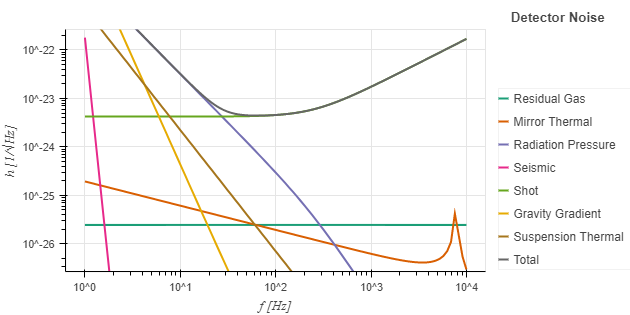
\includegraphics[scale=0.55]{SPQMaxNoLim.png}
    \captionsetup{width=0.9\textwidth}
    \caption{One combination of parameters that return maximum
      sensitivity without budget or complexity limits. The quantum
      noise curves limit detector sensitivity, meaning that parameters
      not included in these noises can vary over a wide range without
      changing the overall detector sensitivity.}
    \label{fig::SPQMaxNoLim}
\end{figure}

An optimisation including the budget and complexity was also
implemented, returning 203 detections. As expected, this was found at
a combination compromising truly optimal values, due to the added
limits. The true parameters achieving this high score will not be
revealed in this document. 
This was found to be approximately at depths below 20m, $N_p$ ranging
from (7-8)km$^{-1}$, $T$ from (55-63)K, $l$ from (1.8-2.0)m,  $M$ from
(81-82)kg, $P$ from (47-53)W, $r$ from (1-1.2)nm and $N_s$ = 3. These
values will be commented out when this document is released
externally. 


\subsection{Effects of Mirror Material and Location Choices}
As location and mirror material were not varied in the MCMC, the
effects of these variables were tested independently. 

\textbf{Mirror material}: Silicon, Silica and Sapphire have the same
values of mechanical damping factor, $\mathcal{L}$, but are
distinguished by differing optical losses. This is outlined in
appendix \ref{app::material}. Lower optical loss means greater mirror
quality factor $\mathcal{Q}$, leading to lower mirror thermal
noise. This increases the sensitivity of the detector, leading to a
greater detector range and number of detections. 

According to this logic, Silicon should return the greatest detector
range, followed by Sapphire and then Silica. Crystal appears to have
the greatest optical loss, which leads to significantly greater mirror
thermal noise as shown in figure \ref{fig::aLIGOSiliconCrystal}. It
also has a lower value of $\mathcal{L}$, which increases shot noise
and reduces radiation pressure noise slightly, as well as reducing
complexity. Consequently, selecting this material should lead to the
lowest detector range and therefore number of detections. This was
tested by setting the parameters to those for the aLIGO model
(including Island for location), and varying the mirror materials. The
results are detailed in table \ref{tab::materialstest}, confirming
what is expected. 
%\begin{enumerate}
%\item \textbf{Silicon}: Returns the highest number of detections and highest score, which is expected when considering that it has the lowest optical losses. This is reflected in equations \ref{eqn::qsapp} through to \ref{eqn::qsilica}. Lower optical loss means greater mirror quality factor, leading to lower mirror thermal noise. This increases the sensitivity of the detector, leading to a greater detector range and number of detections. means higher power in the detector arms, leading to less radiation pressure noise.
%The second lowest lossy material is Sapphire, which correspondingly returns the second highest number of detections. Crystal has the highest loss values, therefore returning the least amount of detections. A comparison of the noise produced for the aLIGO model when setting the mirror material to Silicon and Crystal are shown in figure \ref{fig::aLIGOSiliconCrystal}. It is clear that although Crystal is less expensive, it dramatically decreases the sensitivity of the detector across a large range of frequencies.  
%\end{enumerate}

    \begin{table}[h]
    	\centering
  \captionsetup{width=0.9\textwidth}
         \caption{Results obtained for different material choices with
           the aLIGO model. Silicon produces the greatest detector
           range, followed by Sapphire and Silica. Crystal clearly
           leads to the worst overall detector sensitivity, outputting
           no detections.}
    \begin{tabular}{ |c|c|c|c|c| } 
     \hline
     \textbf{Material:} & \textbf{Sapphire}  & \textbf{Crystal}  & \textbf{Silicon}  & \textbf{Silica} \\ 
     \hline
     \textbf{$N_{bhbh}$}  & 2 & 0 & 2 & 2\\ 
     \hline
     \textbf{$N_{nsns}$}  & 6 & 0 & 6 & 5\\ 
     \hline
     \textbf{$N_{sn}$}  & 1 & 0  & 1 & 1 \\ 
     \hline
     \textbf{$r_{bhbh}$ (Mpc)}  & 653.07 & 58.57  & 657.35  & 644.92 \\ 
     \hline
      \textbf{$r_{nsns}$ (Mpc)}  & 138.54  & 4.95  & 142.74 & 131.37 \\ 
      \hline
    \textbf{Score (Mpc)}  & 153.16  & 7.67  & 157.15  & 146.35 \\
    \hline
    \textbf{Total Cost (\$)}  & 68879252  & 57939252  & 63999252  & 61979252 \\ 
    \hline
      \textbf{Total Complexity}  & 18.02  & 17.42  & 18.02  & 18.02 \\ 
     \hline
    \end{tabular}
    \label{tab::materialstest}

    \end{table}
    
\begin{figure}
\centering
\begin{subfigure}{.8\textwidth}
        \centering
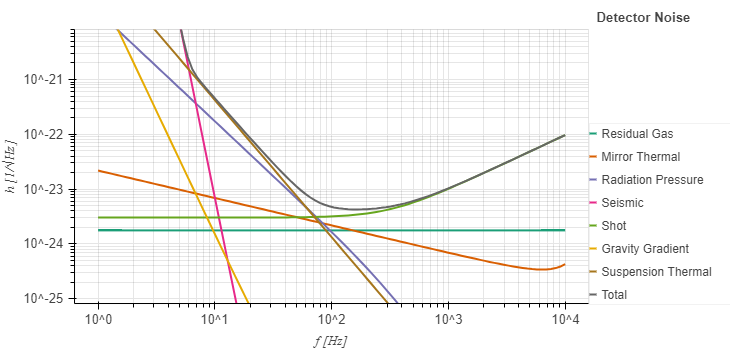
\includegraphics[width=1\linewidth, trim = {0 0 0 1cm}, clip]{aLIGOSilicon.png}
         \caption{Silicon}
         \label{fig::PowerStages}
         \end{subfigure}%\hfill 
         \\
        \begin{subfigure}{.8\textwidth}
        \centering
        \includegraphics[width=1\linewidth, trim = {0 0 0 0.9cm}, clip]
         {{aLIGOCrystal.png}}
\caption{Crystal}
         \label{fig::PowerStagesMass}
         \end{subfigure}
         \caption{Comparison between effects of Silicon and Crystal
           mirror materials on the detector sensitivity. The selection
           of Crystal greatly increases mirror thermal noise, in turn
           decreasing the sensitivity of the detector across a large
           range of frequencies. It also slightly reduces radiation
           pressure noise and increases shot noise.}
         \label{fig::aLIGOSiliconCrystal}
 \end{figure}

\textbf{Location}: The values correspond to location are detailed in
appendix \ref{sec:sites}. Desert has the least mechanical
susceptibility scaling $X_{dc}$ and high frequency floor $X_{hf}$, as
well as the greatest exponent to the frequency-dependent scaling
$n_0$. It is based on a mixed spectrum of globally seismic
sites. According to equation \ref{eqn::baseseismic}, this location
should result in the lowest values of seismic and gravity gradient
noise. By contrast, City has high values of $X_{dc}$ and $X_hf$, as
well as the lowest value of $n_0$, meaning that it should output the
maximum seismic and gravity gradient noise and therefore smallest
detector range. Island and Jungle fall in the middle of these two
location in terms of minimising noise. Island has a lower value of
$X_{dc}$ and higher $n_0$ than Jungle, but also a greater
$X_{hf}$. This makes it difficult to deduce which of the two would
result in a greater detector range. 

Again setting the initial values to the aLIGO model (including Silica
for mirror mass), the location was varied, and the results can be seen
in table \ref{tab::locationtest}. The results for Island are the same
as for Silica above as the parameter combinations are identical, but
it is repeated for completeness. As expected, Desert and City return
the greatest and smallest detector range respectively. The detector
ranges for Jungle and Island fall in the middle as predicted, with
Jungle appearing to be a slightly better option as it gives a greater
detector range. The total number of detections does not vary as the
ground motion noises are predominant at low frequencies and does not
have a large effect with the selected source masses. A comparison
between the Desert and City locations can be seen in figure
\ref{fig::aLIGODesertCity}. Setting the City location increases
seismic and gravity gradient noises, leading to a lower detector
sensitivity. 
    
    \begin{table}[h!]
    \centering
    \captionsetup{width=0.9\textwidth}
    \caption{Results obtained for different location choices. As
      change in location only has an effect at low frequencies, the
      total number of detections remains the same at all
      locations. However, the Desert location maximises the range of
      the detector, followed by Jungle then Island. The high ground
      motion noise with City means it has the smallest detector
      range.}
    \begin{tabular}{ |c|c|c|c|c| } 
     \hline
     \textbf{Site:} & \textbf{City}  & \textbf{Jungle}  & \textbf{Desert}  & \textbf{Island} \\     \hline
     \textbf{$N_{bhbh}$}  & 2 & 2 & 2 & 2\\ 
     \hline
     \textbf{$N_{nsns}$}  & 5 & 5 & 5 & 5\\ 
     \hline
     \textbf{$N_{sn}$}  & 1 & 1  & 1 & 1 \\ 
     \hline
     \textbf{$r_{bhbh}$ (Mpc)}  & 643.51 & 645.03 & 645.16  & 644.92 \\ 
     \hline
     \textbf{$r_{nsns}$ (Mpc)}  & 131.34  & 131.37  & 131.38 & 131.37 \\ 
     \hline
    \textbf{Score (Mpc)}  & 146.26  & 146.36  & 146.36  & 146.35 \\ 
    \hline
    \textbf{Remaining Budget (\$)}  & 33020748  & 63020748  & 23020748 & 43020748 \\ 
    \hline
    \end{tabular}
    \label{tab::locationtest}
    \end{table}
    
    
    \begin{figure}[h!]
\centering
\begin{subfigure}{.8\textwidth}
        \centering
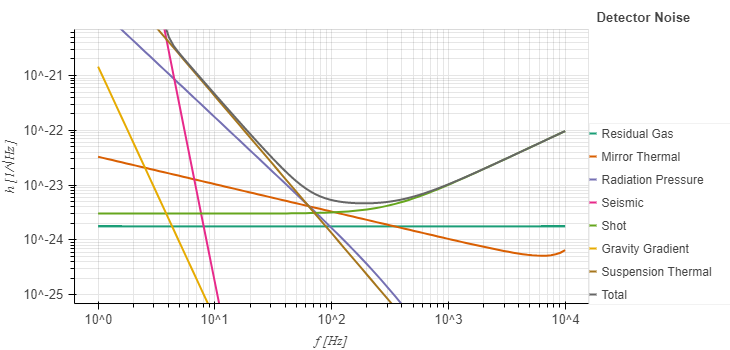
\includegraphics[width=1\linewidth, trim = {0 0 0 1cm}, clip]{aLIGODesert.png}
         \caption{Desert}
         \label{fig::PowerStages}
         \end{subfigure}%\hfill 
         \\
        \begin{subfigure}{.8\textwidth}
        \centering
        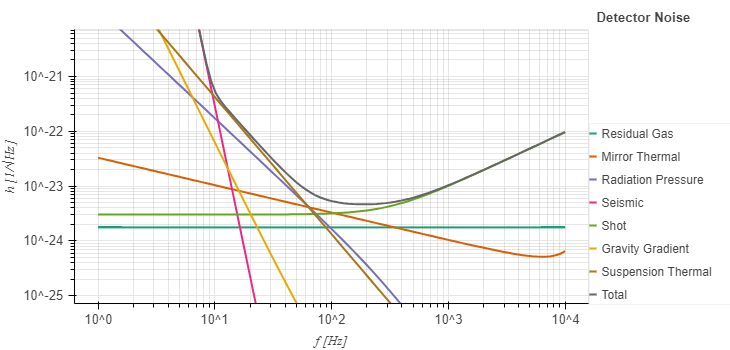
\includegraphics[width=1\linewidth, trim = {0 0 0 0.9cm}, clip]{aLIGOCity.png}
\caption{City}
          \label{fig::aLIGODesertCity}
         \end{subfigure}
         \caption{Comparison between effects of Desert and City
           locations on the detector sensitivity. Selecting City leads
           to an increase in both seismic and gravity gradient
           noise. However, the effect on the total noise curve is over
           a small range at a low frequency, meaning that the overall
           detector range and sensitivity does not alter
           significantly}
         \label{fig::aLIGOSiliconCrystal}
 \end{figure}
 
 The complexity of the materials and the costs for both match up to
 the values selected for the game outlined in the appendices (the
 complexity does not change with location, it remains constant at
 18.02). 

\subsection{Frequency Band Sensitivity}
\label{sec::fband}
Gravitational wave detectors can be optimised for different frequency
bands to detect selected sources. Currently, detector sensitivity is
greatest in the range of (10-10$^3$)Hz. Compact binary inspirals
release gravitational waves in the form of sinusoids, increasing in
frequency and amplitude until the end of the inspiral phase. They
spend a variable amount of time in different frequency bands. A
neutron star binary inspiral, with each neutron star assumed to be a
mass of 1.4M$\odot$, will have a maximum gravitational wave frequency
of 1500Hz \cite{LIGO}. Inspirals of higher mass terminate at
proportionally lower frequencies. As neutron stars are less massive
than black holes, setting parameters to achieve greater sensitivity at
a high frequency band should return more detections of neutron
stars. This property was checked for Space Py Quest as described
below. 

Again setting the parameters to mirror the aLIGO model, the power was
increased to 200W. This decreased shot noise, which dominates at
higher frequencies, and returned detections of five neutron star
binaries, one black hole binary and one supernova. 

The parameters were then varied to favour greater sensitivity at a
lower frequency. This involved moving the power down to 7W to increase
shot noise and reduce radiation pressure, changing location to Desert
to reduce seismic and gravity gradient noise, and increasing
suspension length and mirror mass to their maximum values, mostly to
reduce radiation pressure and suspension thermal noises. The resulting
noise curves can be seen in figure \ref{fig::LowHighFreq}. This output
three neutron star binaries, 32 black hole binary and zero supernova
detections. As one supernova detection has been included for a good
mid-high frequency range sensitivity, Space Py performs as expected in
different frequency bands. 

    \begin{figure}[h!]
\centering
\begin{subfigure}{.8\textwidth}
        \centering
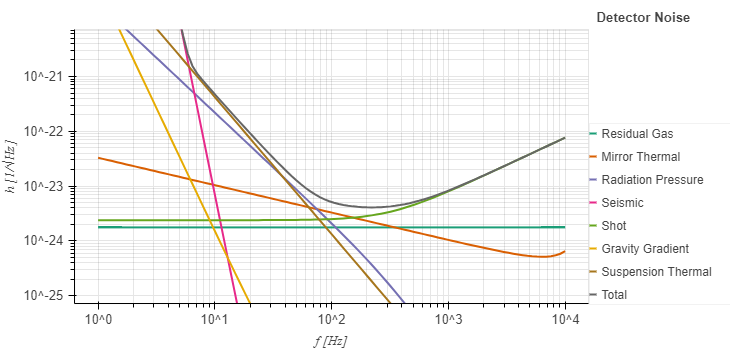
\includegraphics[width=1\linewidth, trim = {0 0 0 1cm}, clip]{HighFreq.png}
         \caption{Optimising for high frequency range}
         %\label{fig::PowerStages}
         \end{subfigure}%\hfill 
         \\
        \begin{subfigure}{.8\textwidth}
        \centering
        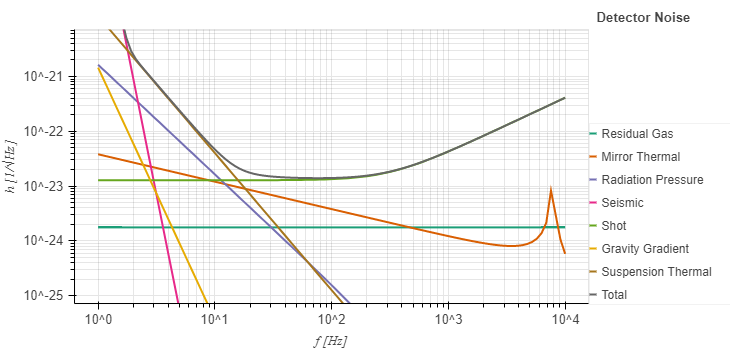
\includegraphics[width=1\linewidth, trim = {0 0 0 0.9cm}, clip]
{LowFreq.png}
         \caption{Optimising for low frequency range}
          %\label{fig::aLIGODesertCity}
         \end{subfigure}
         \caption{Sensitivity curves obtained when optimising for
           different frequency ranges. Optimising for higher
           frequencies means that high frequency sources like neutron
           stars and supernovae are more likely to be detected. Black
           holes signals terminate at lower frequencies, making them
           more likely to be found when optimising for low frequency.}
         \label{fig::LowHighFreq}
 \end{figure}

%\clearpage
\section{Discussions and Outlook}
\subsection{Conclusions of Testing}
 The primary checks carried out on Space Py Quest all appear to
 indicate that it behaves as intended. The discrepancies found between
 the original Space Py Quest have been investigated and documented,
 and the output noise curves scale with the relevant parameters as
 expected. The parameters outputting the maximum sensitivity for total
 number of detections is also as expected from the noise equations
 used in the game. Finally, it detects more neutron star binaries for
 a greater sensitivity at high frequency, and more black hole binaries
 for a greater sensitivity at a lower frequency, as it should. The
 testing henceforth has not revealed any major problems that need to
 be changed in this game. 
 
\subsection{Ideas for the Future}
\label{sec:discussion}
Space Py Quest was built in a limited time frame and is a work in
progress. Some thoughts on possible steps forward are detailed below.
\begin{enumerate}
\item \textbf{Narrative}\\
It is realistic that detector designs be swiftly modified and the
results of these modifications considered. It is somewhat realistic
that a detector could be modified after one observing run in order to
make improvements. However, it is not realistic that the whole
kilometer-scale detector could be picked up and moved to a different
location. In order to make Space Py Quest's narrative and aims more
similar to those of Space Time Quest, future versions of the game
could limit users to 5 or so `upgrades'. Additionally, putting the
location specification widget in a preceding Jupyter notebook
container would add some semblance of a one-way narrative. 
\item \textbf{Themed Parameters} \\
    During the `design phase' of Space Time Quest, the user can switch
    between 3 sets of parameters, each with a certain theme or
    `subsystem': Environment, Vibration Isolation and Optics. Space Py
    Quest currently has just one drop-down menu from which all of the
    parameters can be accessed. This was done to test user addition of
    additional variables. It was also extremely easy to do using the
    dictionary of detector parameters. The parameters could instead be
    held in themed tabs to segregate them into subsystems, making the
    interface more similar to Space Time Quest. 
\item \textbf{Leaderboard or Prize} \\
    There is not the same motivation for a user to obtain the largest
    range in Space Py Quest as there is in Space Time Quest. There is
    only scientific curiosity, which is perhaps \textit{more}
    well-satisfied in Space Py Quest, as the result of the science run
    is more informative about specific sources. To be used a teaching
    tool for younger students, there could perhaps be a more
    accessible motivation, like a leaderboard or a printable
    certificate.
\item \textbf{Showcasing Resonance} \\
Including slightly more accurate noise equations for things like
mirror thermal noise would enable the curves to spike at resonant
frequencies. The origins of these spikes may be  too advanced for
certain levels of education, but could be something to investigate
when used as a teaching tool, as it has a visual effect on the noise
curves that may be peculiar to someone unfamiliar with the underlying
physics.
        \item \textbf{User Definition of New Noise} \\
    In the package containing Space Py Quest is a file named
    $translate.py$. The functions in this file create a key to define
    new noise functions in terms of detector variables, generate new
    noise classes in a separate script, and import these new classes
    so that they can be passed to the score calculator. The new noise
    curves are then added to the existing noise plot, with an
    embedded, user-defined tag to denote their nature. This does not
    make up part of the game yet, but could be investigated by users,
    or included at a later date.
    \item \textbf{Detector Distance Calculation}\\
    The detector distance calculation considers the inspiral section
    of binary merger signals only. This means that the high-frequency
    sensitivity of the detector is actually irrelevant to the range
    reported, which is not physically realistic, and could end up
    teaching users incorrect physics. The shape of the
    frequency-domain signal could be approximated for a game like
    Space Py Quest very simply. 

    \begin{figure}
    \centering
    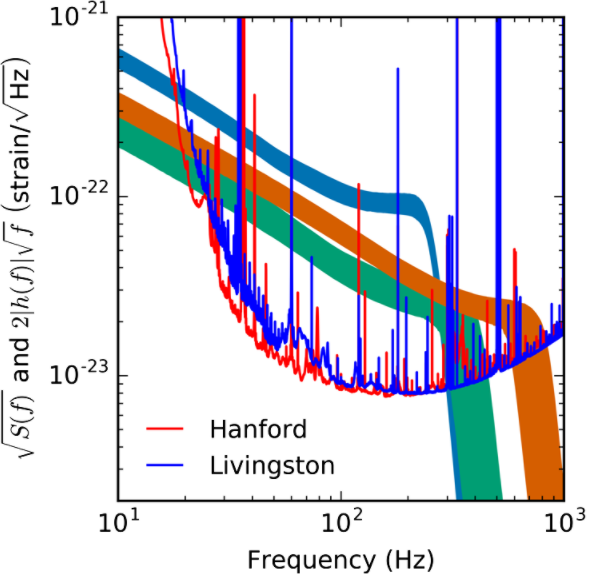
\includegraphics[scale=0.6]{fdomsig.PNG}
    \caption{Frequency domain signals for detections GW150914 (blue),
      LVT151012 (green) and GW151226 (orange). These exact signals are
      nontrivial to recreate, but can be approximated fairly simply by
      splitting into 3 sections with different
      gradients. \cite{binary}}
    \label{fig:fdomsig}
    \end{figure}
Frequency domain signals from the first 3 detections made by the LIGO
collaboration are shown in figure \ref{fig:fdomsig}. Phenomenological
models, such as IMRPhenomB, generate very nearly accurate frequency
domain gravitational waveforms. Doing this within Space Py Quest would
be considerably more complex than required to provide a relatively
realistic estimate of a detector range calculation.

The IMRPhenomB model proposed by Ajith \textit{et al.} \cite{ajith}
uses three transitional frequencies to indicate at which stage in the
merge a point within the binary signal has been emitted. Each make use
of a conversion factor,
\[
conv = \frac{GM_{\odot}}{c^2}.
\]
The first, $f_{merge}$, describes the point at which the inspiral
stage becomes the actual coalescence. The signal gradient up until
this point is well-approximated within Space Py Quest. This can be
simplified for the game from its value in Ajith:
\[
f_{merge} = (1 - 4.455 + 3.521) \times conv \approx 0.07 \times conv .
\]
The coalescence moves from the merge to the ringdown stage at a frequency
\[
f_{ring} = \frac{1 - 0.63}{2} \times conv \approx 0.19 \times conv,
\]
and the cutoff frequency can be given by
\[
f_{cutoff} = 0.3236 \times conv \approx 0.32 \times conv.
\]
Using these transition frequencies, a very simple inspiral waveform
can be constructed using the shallow inspiral slope already calculated
in Space Py Quest until $f_{merge}$, a horizontal line at this
amplitude from $f_{merge}$ to $f_{ring}$, and then a steeper slope
from $f_{ring}$ to $f_{cutoff}$. 
\end{enumerate}

\subsection{A Personal Note}
It may interest a reader to know that Space Py Quest was originally
built as a training exercise towards the creation of a software
package for performing full, non-simplified noise calculation for
ground-based gravitational wave interferometers, called MAGIC. To this
end, the making and testing of Space Py Quest has been an invaluable
learning curve. We have discovered the benefits of using Python's
$dictionary$ type to make dynamic, quickly-modified models whose
parameters are portable and easily inserted into testing methods. This
has directly translated into the setup of our detector classes in
MAGIC. Python's capacity for list comprehension has also significantly
influenced our approach to our new noise calculation software, which
we intend to be as efficiently written as possible. Space Py Quest is
essentially a toy model of MAGIC, and the lessons learnt in
constructing and using the game have both consciously and
unconsciously weighted the procedures with which we construct and test
the latter.

%\clearpage
\begin{appendix}
\section{Appendix}
Any symbols used within equations in this document that have a fixed
value throughout the game are given in this section, in addition to
any other functions that have not yet been noted.

\subsection{Utility Function}
There is only one utility function, which returns the result of a
linear interpolation between points $y(x)$ at point $x = t$. If $t$
falls between points $x_i$ and $x_{i+1}$, then the returned value is
\begin{equation}
    \mathcal{I}(x, y, t) = y(t) = \frac{y_i(x_{i+1} - t) + y_{i+1}(t - x_i)}{x_{i+1} - x_i}.
    \label{eq:lerp}
\end{equation}
\subsection{Global Constants}
\label{sec:constants}
\begin{center}
    \begin{tabular}{ |c|c|c| } 
     \hline
     \textbf{Name} & \textbf{Symbol}  & \textbf{Value}\\     
     \hline
     Speed of light  & $c$ & $299792458$ ms$^{-1}$\\ 
     \hline
     Newton's gravitational constant  & $G$ & $6.67408 \times 10^{-11}$\\ 
     \hline
     Gravitational acceleration at Earth  & $g$ & $9.81$ ms$^{-2}$\\ 
     \hline
     Mass of the Sun  & $M_{\odot}$ & $1.99 \times 10^{30}$ kg\\ 
     \hline
     Planck's constant  & $h$  & $6.626068 \times 10^{-34}$ kgm$^2$s$^{-1}$\\ 
     \hline
    Boltzmann constant  & $k_b$  & $1.380650 \times 10^{-23}$ JK$^{-1}$\\ 
    \hline
    Atmospheric pressure  & $\mathcal{P}$  & $1013$ mbar\\ 
    \hline
    Temperature of Nitrogen  & $T_N$  & $77$ K\\ 
    \hline
    Radius of the Earth & $R_E$ &  $6400$ km\\ 
    \hline
    Astronomical unit & $au$ &  $149598000$ km\\ 
    \hline
    Megaparsec & $Mpc$ & $3.08568025 \times 10^{22}$ km\\ 
    \hline
    \end{tabular}
\end{center}

\subsection{Detector Constants}
Detector parameters that cannot be altered through the Jupyter
notebook interface are provided below, with examples are given from
VIRGO and/or aLIGO \cite{advLIGO}\cite{VIRGO}.
\begin{center}
    \begin{tabular}{ |c|c|c|c| } 
     \hline
     \textbf{Name} & \textbf{Symbol}  & \textbf{Value} & \textbf{Note}\\     
     \hline
     Detector arm length & $L$ & 5000 m &
            VIRGO arm length: 3000 m\\
     & & &  aLIGO arm length: 3994.5 m\\ 
     \hline
     Detector finesse & $\mathcal{F}$ & 60 &
            VIRGO finesse: 50\\
     & & &  aLIGO finesse : 450\\ 
     \hline
     Laser wavelength & $\lambda$ & $1064 \times 10^{-9}$  & VIRGO 		laser wavelength: 1064$ \times 10^{-9}$ m\\
     & & &  aLIGO laser wavelength: $1064 \times 10^{-9}$ m \\
     \hline
     Detector power recycling factor & $F_{PR}$ & 100 &
            VIRGO power recycling factor: 50\\
     & & & aLIGO power recycling factor: 43.61\\ 
     \hline
     First mirror resonance & $f_R$ & 4000 Hz &
      VIRGO first mirror resonance: $\approx$ 5600 Hz\\ 
     \hline
     Cost of each vacuum pump & $C_v$ & \$850000 & \\ 
    \hline
    Initial ambient temperature & $T_0$ & 300 K &
            VIRGO ambient temperature: 300 K\\
     & & &  aLIGO ambient temperature: 290 K \\
    \hline
    Temperature increase per kilometer & $ \Delta T$ & 30 K & \\
    Depth array & $ \mathbf{d} $ & $[0, 10, 100, 500]$ m & \\ 
    \hline
    Complexity array & $ \mathbf{Z}_d$ & $ [0, 1, 4, 6]$ &\\ 
    \hline
    \end{tabular}
\end{center}

\subsection{Ranges}
\label{sec:ranges}
User-modifiable variables must be restricted to within physically
realistic limits. Those enforced by Space Py Quest are given in the
table below. Some information is provided to justify the choice of
range \cite{advLIGO}\cite{VIRGO}.
\begin{center}
    \begin{tabular}{ |c|c|c|c| } 
     \hline
     \textbf{Name} & \textbf{Symbol}  & \textbf{Range} & \textbf{Note}\\     
     \hline
     Frequency range  & $f$ & $[10^{-4}, 10^5]$ Hz & aLIGO and VIRGO frequency ranges: \\ 
     &  &  &  $\sim 10^0 - 10^4$ Hz\\
     \hline
     Detector burial depth & $d$ & $[0, 1000]$ m & Both VIRGO and aLIGO are above ground, \\
     & & & but future detectors like the Einstein \\
     & & & Telescope (ET) could be buried \\ 
     & & & 100 - 200 m underground \cite{ET}.\\ 
     \hline
     Number of vacuum pumps & $N_p$ & $[0, 16]$ &
            The number of vacuum pumps influences \\
     & & &  the pressure in the interferometer arms, \\
     & & & as calculated using equation \ref{eq:pressure}.\\ 
     \hline
     Detector temperature & $T$ & $[1, 330]$ K &
            VIRGO suspension temperature: 300 K\\
     & & & aLIGO suspension temperature: 300 K\\ 
     \hline
     Number of suspension stages & $N_s$ & $[1, 9]$ & 
            Both VIRGO and aLIGO have 4 suspension stages.\\ 
     \hline
    Suspension length & $l$ & $[0.35, 5]$ m &
            VIRGO suspension length: 0.7 m \\
    & & & aLIGO suspension length: $\sim 0.5$ m\\ 
    \hline
    Mirror mass& $M$ & $[5, 100]$ kg &
            VIRGO mirror mass: $\sim 20.4$ kg\\
    & & & aLIGO mirror mass: $\sim 40$ kg\\ 
    \hline
    Laser power & $P$ & $[1, 200]$ W &
            aLIGO laser power: 125 W\\ 
    \hline
    Mirror surface roughness& $R$ & $[1, 500]$ nm &
            aLIGO mirror surface quality: $\sim 0.1$ nm\\ 
    \hline
    \end{tabular}
\end{center}

\subsection{Site-dependent Values}
\label{sec:sites}
\begin{figure}
        \centering
        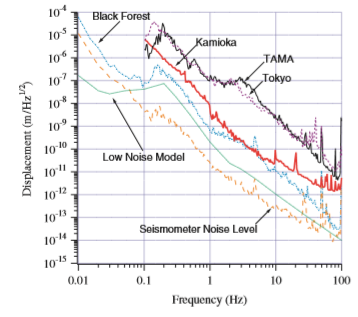
\includegraphics{noisecurves.PNG}        
\caption{Seismic noise curves for Kamioka, TAMA300 site, Tokyo, Black
  Forest Geophysical Observatory in Germany, and a hybrid low noise
  model build from data from global quiet sites, as plotted by Ohashi
  \textit{et al.}(2003) \cite{CLIO}.}
        \label{fig:ohashi}
    \end{figure}
    The detector site influences the seismic noise curve, budget and
    complexity. The seismic noise is an approximation of the noise
    curves shown in figure 7 of Ohashi \textit{et al.}(2003)
    \cite{CLIO}, which is reproduced in figure \ref{fig:ohashi} in
    this document. $City$, $Island$ and $Jungle$ come close to the
    curves for Tokyo, Kamioka and the Black Forest in order, whilst
    $Desert$ is a mixed spectrum of global seismically quiet
    sites. Each $site$ class defines 6 identically-named data
    members. The data members include \textit{Complex Credits}, a
    scaling parameter for complexity, and \textit{Budget}, the amount
    of money available to the player.
    \begin{center}
    \begin{tabular}{ |c|c|c|c|c|c| } 
     \hline
     \textbf{Name} & \textbf{Symbol} & \textbf{City}  & \textbf{Jungle}  & \textbf{Desert}  & \textbf{Island} \\ 
     \hline
     Complex Credits & $Z_{cred}$ & 20 & 19 & 17 & 18\\ 
     \hline
     Budget & - & $95 \times 10^6$ & $125 \times 10^6$ & $85 \times 10^6$ & $105 \times 10^6$\\ 
     \hline
     Mechanical susceptibility scaling & $X_{dc}$  & $3 \times 10^{-5}$ & $5 \times 10^{-5}$  & $1 \times 10^{-7}$  & $8 \times 10^{-6}$ \\ 
     \hline
     High-frequency floor & $X_{hf}$  & $1 \times 10^{-11}$  & $5 \times 10^{-14}$  & $8 \times 10^{-15}$  & $9 \times 10^{-13}$ \\ 
     \hline
     Critical frequency & $f_c$ & 0.15 & 0.02 & 0.125 & 0.08\\ 
     \hline
     Exponent of frequency-dependent noise scaling& $n_0$  & 2.3 & 2.4 & 2.6 & 2.5\\ 
     \hline
    \end{tabular}
    \label{tab:sites}
    \end{center}
\subsection{Material-dependent Values}
\label{app::material}
Each material has a damping rate, $\mathcal{L}$. Materials with higher
$\mathcal{L}$ contribute less to the mirror thermal noise. It should
be relatively simple for a user to infer that Crystal is $not$ a good
mirror material to choose.
\begin{center}
    \begin{tabular}{ |c|c|c|c|c|c| } 
     \hline
     \textbf{Name} & \textbf{Symbol} & \textbf{Sapphire}  & \textbf{Crystal}  & \textbf{Silicon}  & \textbf{Silica} \\ 
     \hline
     Goodness of losses & $\mathcal{L}$  & 1 & 0.4 & 1 & 1\\ 
     \hline
     Material base cost (\$) & $C_0$  & $4 \times 10^6$ & $5 \times 10^5$ & $2 \times 10^6$ & $1.5 \times 10^6$\\ 
     \hline
     Cost mass scaling (\$) & $A_0$  & $56 \times 10^6$ & $9.5 \times 10^6$  & $38 \times 10^6$  & $28.5 \times 10^6$ \\ 
     \hline
     Temperature data (K) & $\textbf{T} $  & [1, 25, 80,  &  [1, 300 ] & [1, 32, & [1, 35, 90, 150, \\ 
     
      &  & 105, 230, 300 ]  &  & 40, 270, 300 ] & 200, 250, 300 ]  \\ 
     \hline
     Losses data & $\textbf{q}(T)$  & [1.4e-9, 2.5e-8, 7e-9,  & [1e-3, 1e-3 ]  & [1.4e-9, 1.5e-8,  & [1e-3, 7e-4, 1e-4, 3e-6, \\ 
     & & 1.2e-8, 1.6e-8, 1e-7 ]  &  & 7.5e-9, 4.5e-8, 7e-8 ] & 3e-7, 1.5e-7, 1.5e-7 ] \\ 
     \hline
    \end{tabular}
    \label{tab:materials}
    \end{center}
    The total mirror material cost is then
    \begin{equation}
        \mathcal{C}_{mat} = C_0 + A_0\left(\frac{M}{100}\right)^2.
    \end{equation}
\end{appendix}

\clearpage
\bibliographystyle{unsrt}
\bibliography{bibliography}
\end{document}
